\documentclass[a4paper,12pt]{article}
\usepackage[utf8]{inputenc}

\usepackage[top=2cm,bottom=2cm,right=1.5cm,left=1.5cm]{geometry}
\usepackage{amsmath,amssymb,enumitem,multicol,graphicx,tikz,framed,tcolorbox,mathtools,comment,subcaption,array,pgfplots}
\usepackage{listings}
\usepackage{xcolor}
\linespread{1.3}
\setlength\parindent{0pt}
%--------------------------
\usepackage{hyperref}
\hypersetup{
	colorlinks=true,
	linkcolor=blue,
	filecolor=magenta,      
	urlcolor=cyan,
}
%New colors defined below
\definecolor{codegreen}{rgb}{0,0.6,0}
\definecolor{codegray}{rgb}{0.5,0.5,0.5}
\definecolor{codepurple}{rgb}{0.58,0,0.82}
\definecolor{backcolour}{rgb}{0.9,0.9,0.9}
\definecolor{backcolour_two}{rgb}{1,1,1}

\definecolor{kugray5}{RGB}{224,224,224}
\definecolor{linecolor}{RGB}{140,140,140}
\definecolor{shadecolor}{RGB}{180,180,180}

%Code listing style named "mystyle"
\lstdefinestyle{mystyle}{
  backgroundcolor=\color{backcolour},   commentstyle=\color{codegreen},
  keywordstyle=\color{magenta},
  numberstyle=\tiny\color{codegray},
  stringstyle=\color{codepurple},
  basicstyle=\ttfamily\footnotesize,
  breakatwhitespace=false,         
  breaklines=true,                 
  captionpos=b,                    
  keepspaces=true,                 
  numbers=left,                    
  numbersep=5pt,                  
  showspaces=false,                
  showstringspaces=false,
  showtabs=false,                  
  tabsize=2
}

\lstdefinestyle{mystyle_big}{
	backgroundcolor=\color{backcolour_two},   commentstyle=\color{codegreen},
	keywordstyle=\color{magenta},
	numberstyle=\tiny\color{codegray},
	stringstyle=\color{codepurple},
	basicstyle=\ttfamily\normalsize,
	breakatwhitespace=false,         
	breaklines=true,                 
	captionpos=b,                    
	keepspaces=true,                 
	numbers=left,                    
	numbersep=5pt,                  
	showspaces=false,                
	showstringspaces=false,
	showtabs=false,                  
	tabsize=2
}

\lstdefinelanguage{JavaScript}{
	keywords={typeof, new, true, false, catch, function, return, null, catch, switch, var, if, in, while, do, else, case, break, for, let, const},
	keywordstyle=\color{blue}\bfseries,
	%ndkeywords={class, export, boolean, throw, implements, import, this},
	%ndkeywordstyle=\color{yellow}\bfseries,
	identifierstyle=\color{magenta},
	keywords=[2]{ctx},
	keywordstyle=[2]\color{purple}\bfseries,
	keywords=[3]{querySelector, getContext},
	keywordstyle=[3]\color{orange}\bfseries,
	keywords=[4]{class,constructor, export, boolean, throw, implements, import, this, prototype},
	keywordstyle=[4]\color{brown}\bfseries,
	sensitive=false,
	comment=[l]{//},
	morecomment=[s]{/*}{*/},
	commentstyle=\color{gray}\ttfamily,
	stringstyle=\color{red}\ttfamily,
	morestring=[b]',
	morestring=[b]"
}

\lstset{
	language=JavaScript,
	backgroundcolor=\color{lightgray},
	extendedchars=true,
	basicstyle=\footnotesize\ttfamily,
	showstringspaces=false,
	showspaces=false,
	numbers=left,
	numberstyle=\footnotesize,
	numbersep=9pt,
	tabsize=2,
	breaklines=true,
	showtabs=false,
	captionpos=b
}

%"mystyle" code listing set
\lstset{style=mystyle}

\title{Code Listing}
\date{ }
\begin{document}
			\tableofcontents
	\newpage
	\section{Introduction}
	On a basic web page,
	 we can construct and page element called a "canvas". \\
	 It needs a bit of CSS to see what we have done as it begins as an empty transparent rectangle on the page
	\lstinputlisting[language=HTML, caption=Basic Canvas ]{start_js/basic_js.html}
	\begin{figure}[!h]
		\centering
		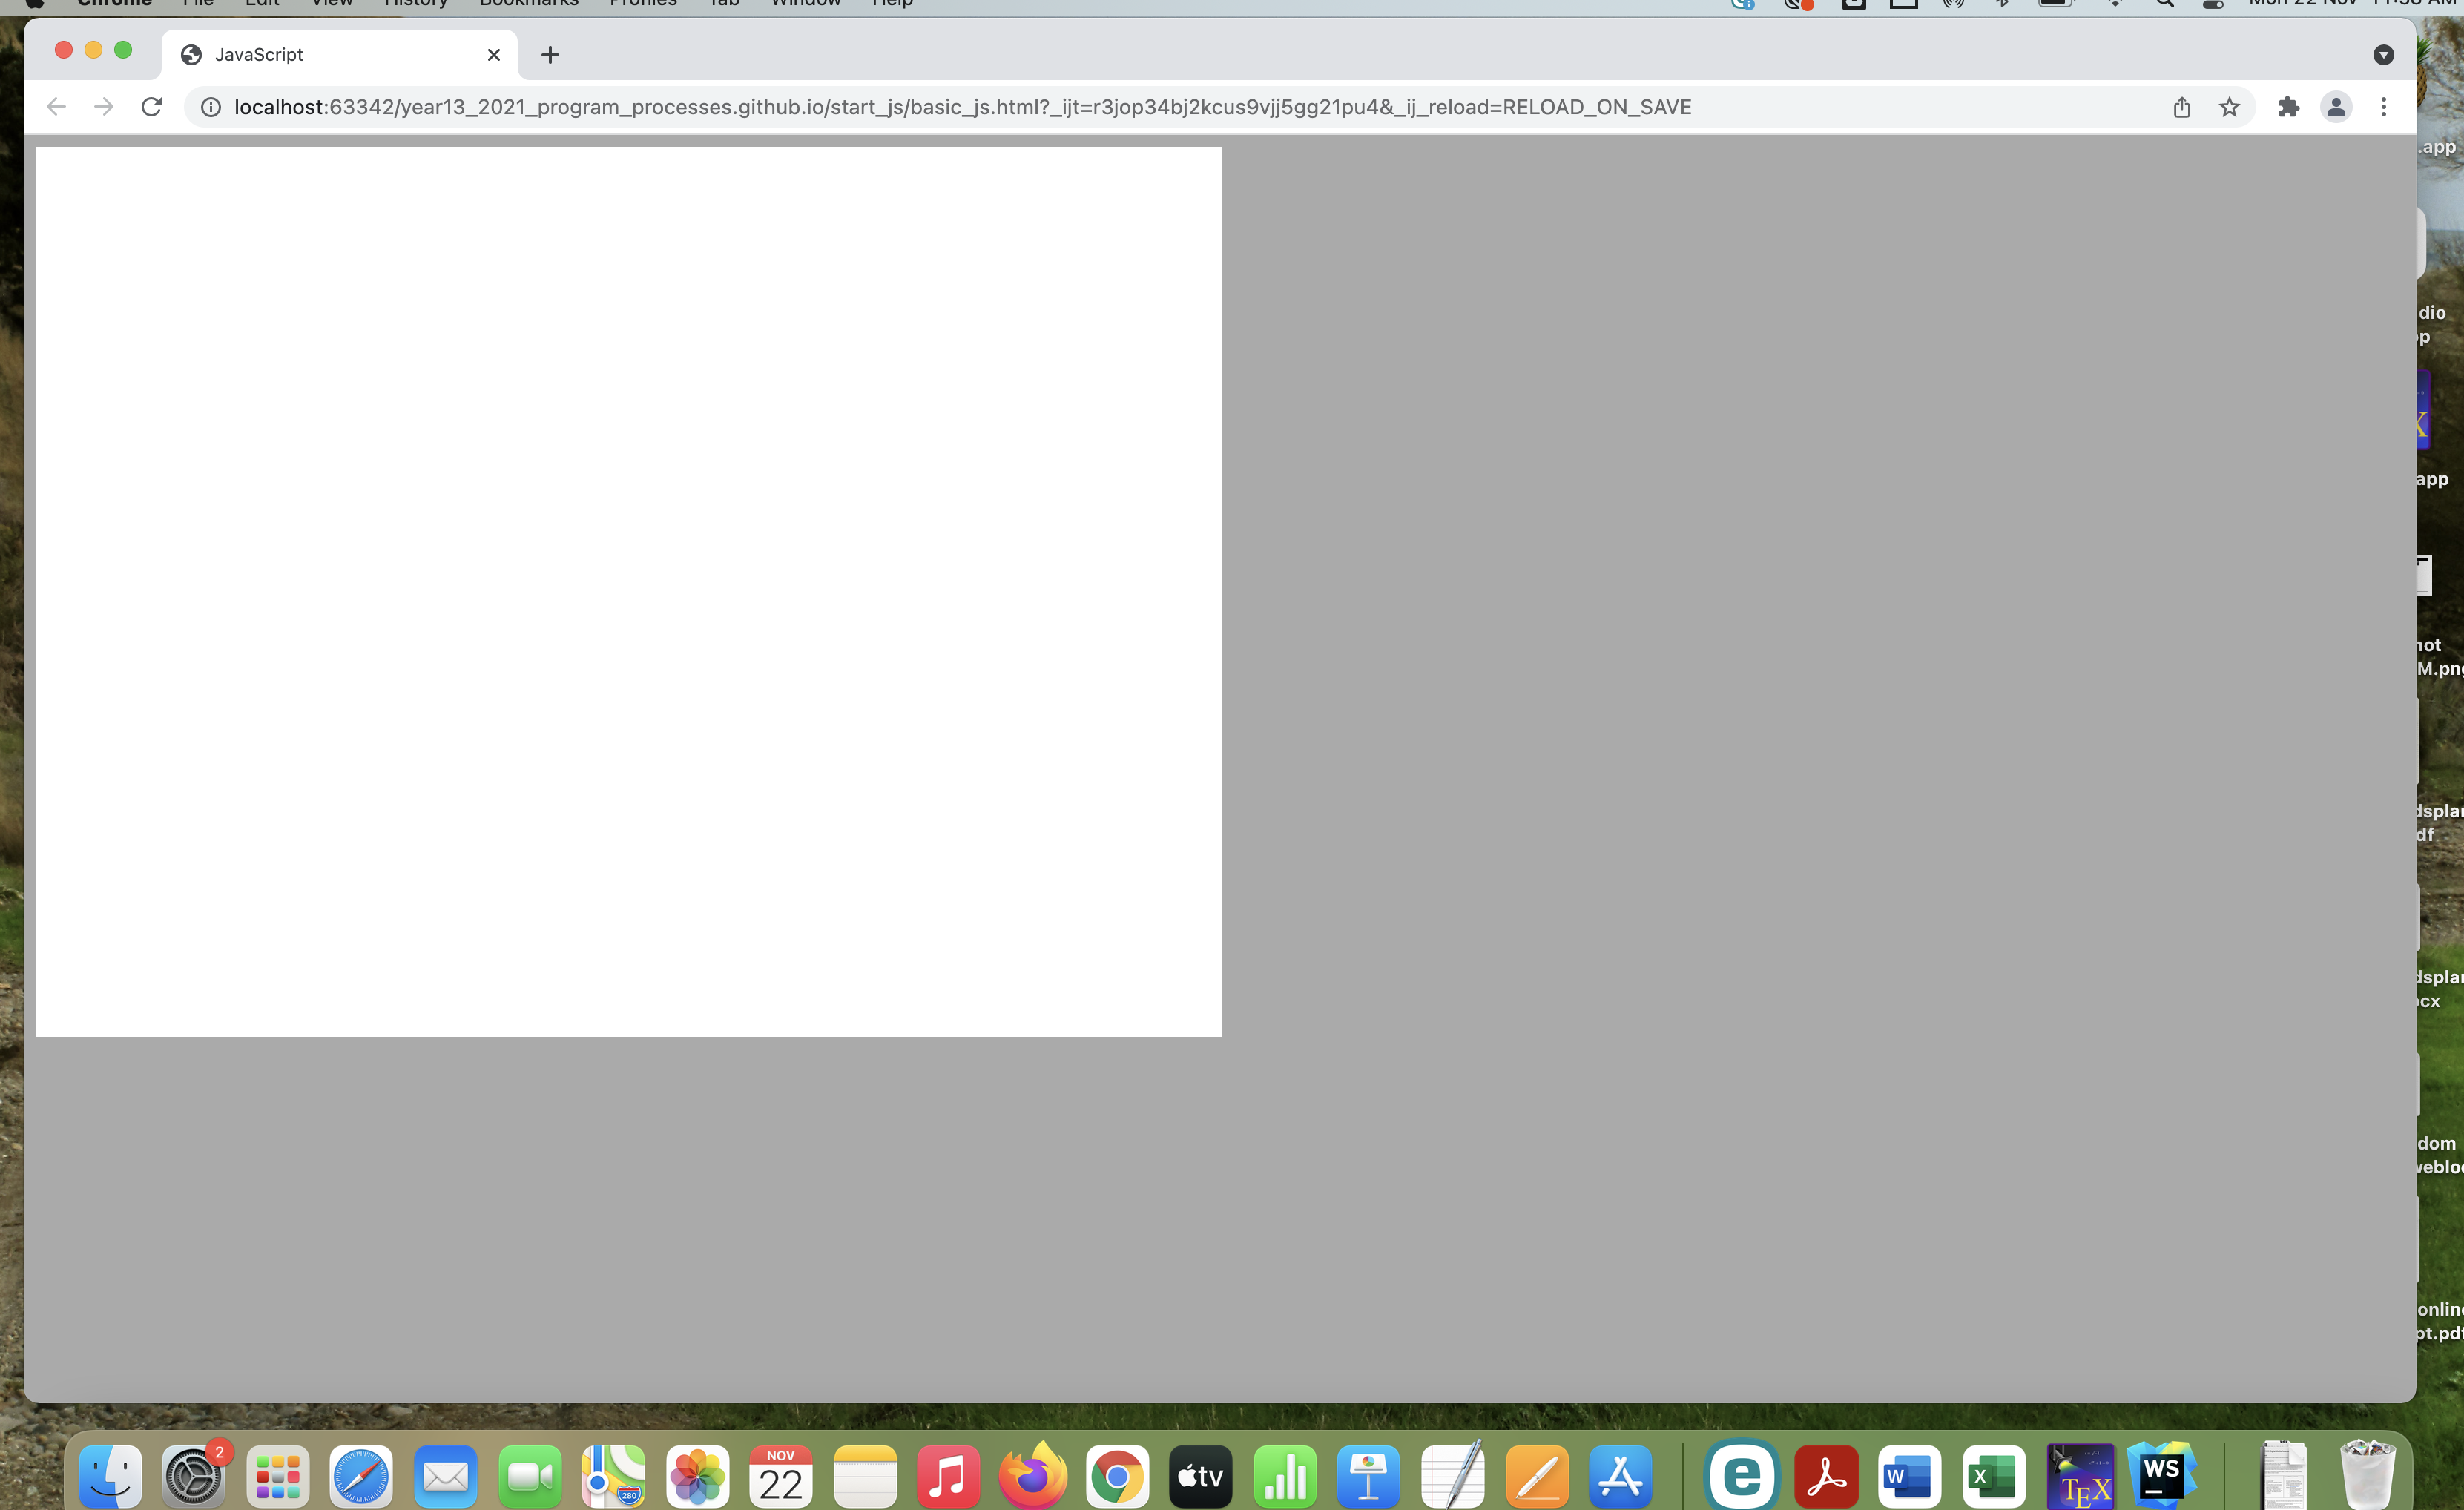
\includegraphics[width=15cm, angle=0, origin=c]{start_js/canvas_in_window.png}
		\caption{Canvas in browser}
	\end{figure}
	\newpage
	The canvas environment allows us to draw shapes and also run animations, so with a bit of work, we are able to create a small web applications such as games or other more interactively rich  experiences.\\
	Our aim is to learn about this environment and to create a small drawing/painting program.\\
\section{Getting started}
To be able to do thing to the canvas we use JavaScript. This is a programming language and in general has many similarities to Python but has some differences in syntax.\\
JavaScript can be written in a web page within the $<$ script $>$ tag.\\
It can also be loaded from an external file (which we will do for most of the unit).
We will have to learn quite a few things about JavaScript as we go through this unit, but regarding drawing shapes, it will always follow the same basic set of steps.
\begin{itemize}
	\item begin a path (i.e the shape)
	\item define the path with its associated parameters (x,y , width, height, ..)
	\item define the fill, stroke and line width (do not need all)
	\item tell the canvas to fill and/or stroke the path
\end{itemize}
\lstinputlisting[language=JavaScript, caption=Basic Shapes ]{start_js/basic_js_draw.html}

This just gives a "general idea" and more complete references:\\
\url{https://www.w3schools.com/html/html5_canvas.asp}\\
\url{https://developer.mozilla.org/en-US/docs/Web/API/Canvas_API}\\
\section{JavaScript in an external file}
It will become quite cumbersome having the JavaScript in the same file as the HTML page.\\
So it is better to have it as a separate file that is linked in.\\
This may make some of the code easier to re-use, as well.
\lstinputlisting[language=HTML, caption=Loading javascript, firstline=12,lastline=13 ]{start_js/basic_js_draw_1.html}
\section{Improving the set up}
It is also helpful to add to the code that connects to that initialises the canvas.\\
The code below can be discussed further, but it allows us the manage the size and basic styling of the canvas from within the JavaScript.
\lstinputlisting[language=JavaScript, caption=Initial JS, firstline=1,lastline=22 ]{functions/rectangle_function.js}

\newpage
\section{Functions}
We can immediately see that even drawing a small number of shapes starts tp build up code, so we want to look at ways of reducing this and having as much as possible available for "re-use".
Let's look at designing a rectangle function and see what we can do with it.\\\\
Picture of design\vspace{10cm}


\lstinputlisting[language=JavaScript, caption=Python example, firstline=24,lastline=62 ]{functions/rectangle_function.js}
\begin{figure}[!h]
	\centering
	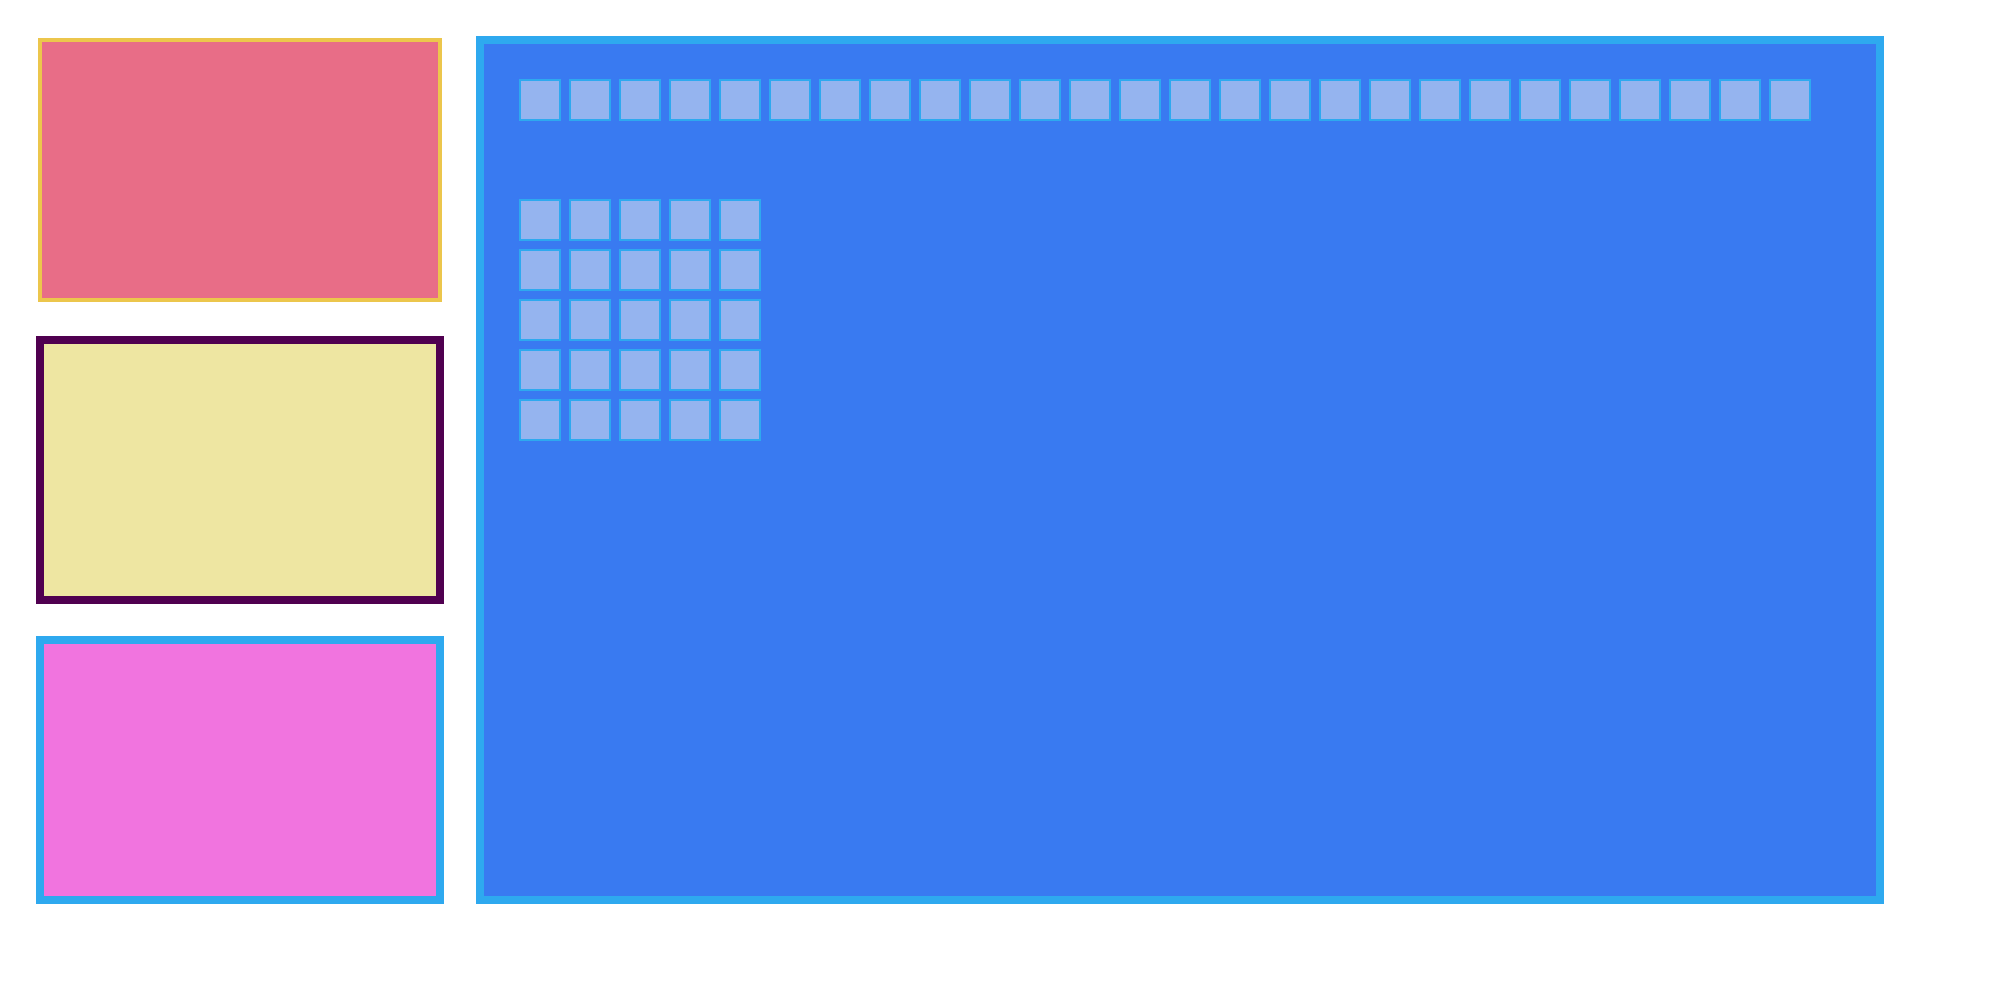
\includegraphics[width=15cm, angle=0, origin=c]{functions/rectangles.png}
	\caption{Canvas in browser}
\end{figure}
Design Functions for:
\begin{itemize}
	\item Circle
	\item Line
	\item Triangle
	\item Square
	\item A Grid
	\item Text Box
\end{itemize}
\begin{figure}[!h]
	\centering
	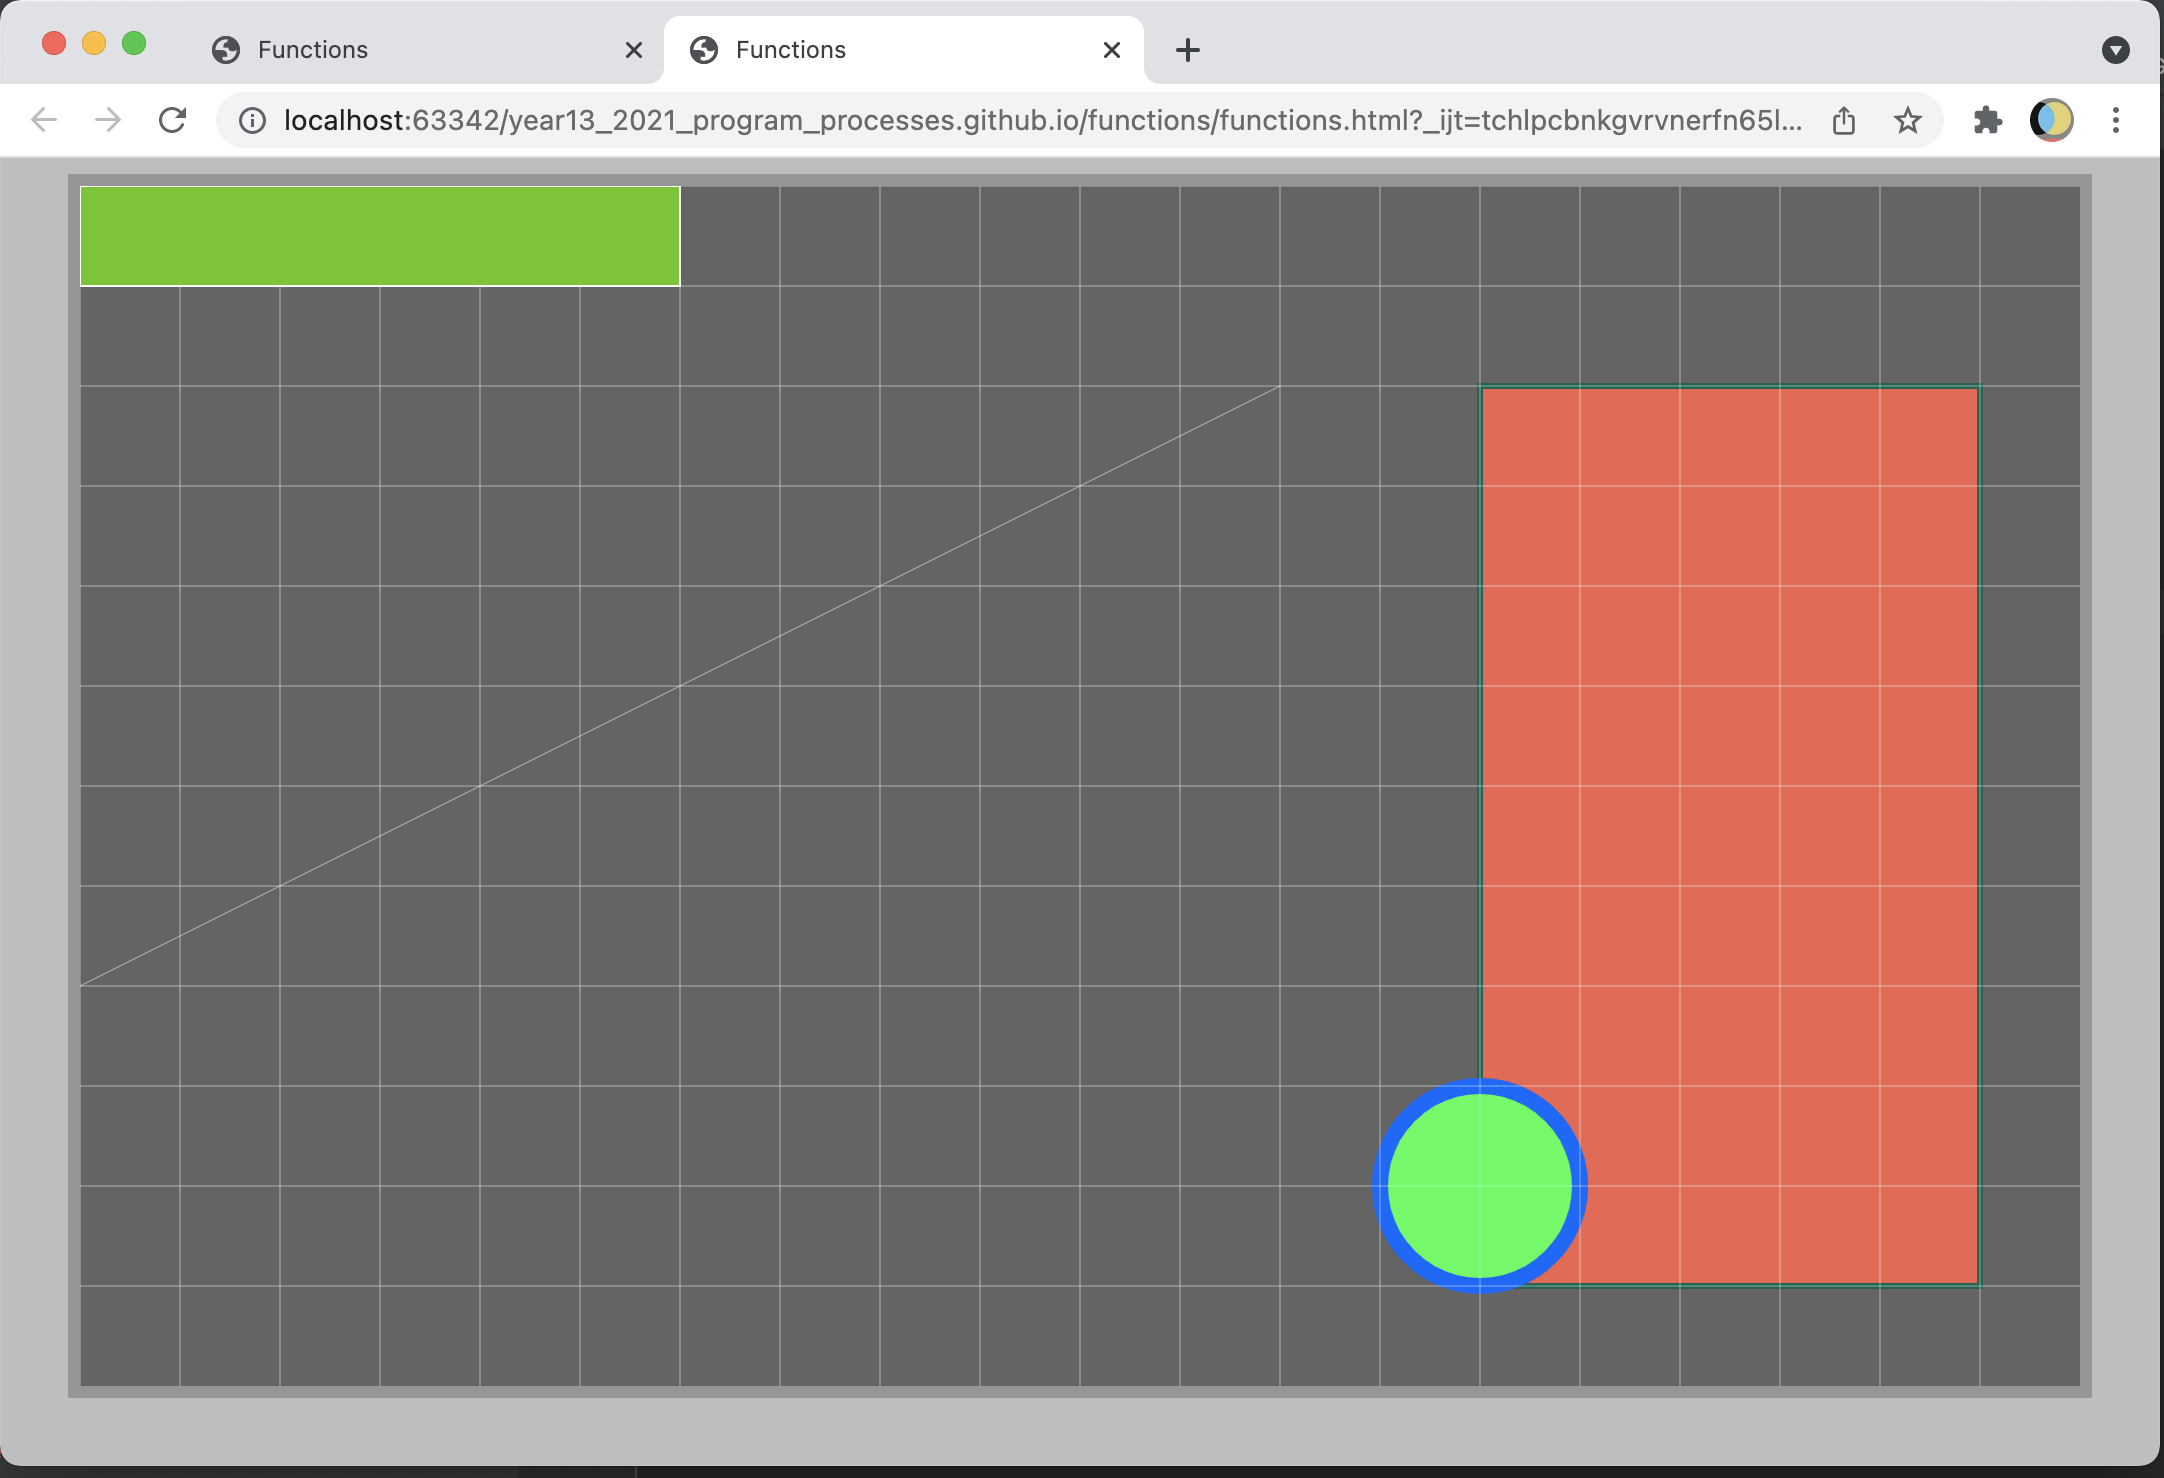
\includegraphics[width=15cm, angle=0, origin=c]{functions/morewithfunctions.png}
	\caption{Canvas in browser}
\end{figure}
\newpage
\section{Making a grid}
\newpage
\section{Update Context Function}
We want to reduce code repetition as much as much as possible.\\
It might be an idea to have a small function to manage the fill and stroke commands.//
This `update context' function can sit near the top of the code and then be called from each of the shape drawing functions.
\lstinputlisting[language=JavaScript, caption=Loading javascript,  firstline=52,lastline=79 ]{functionscollection/init.js}
\newpage
\section{Colour management}
%linerange={1-4,7-9}
Rather than writing the rgb strings all of the time, it might be helpful to start a little colour management data structure.\\
The structure below is actually a simple JavaScript object. But at this stage we can treat much like a Python dictionary.\\
It has a keyword and an associated value.

\lstinputlisting[language=JavaScript, linerange={24-42} ]{colourmanagement/init.js}
We can see its use in the function calls below
\lstinputlisting[language=JavaScript, linerange={66-69} ]{colourmanagement/init.js}
\newpage

\section{Organising an init file}
We probably want to use the functions in various projects (subject to modifications).\\
We also have the set up code.\\
It might be a good idea to assemble this into a separate ``initialisation'' file (aka init.js).
We could then have a separate file that does the ``doing'' of the program.
We can load the files separately into the html document.
\lstinputlisting[language=HTML, caption=Loading javascript ]{functionscollection/index.html}
\lstinputlisting[language=JavaScript, caption=Loading javascript ]{functionscollection/interface.js}
\lstinputlisting[language=JavaScript, caption=Loading javascript ]{functionscollection/init.js}
\begin{center}
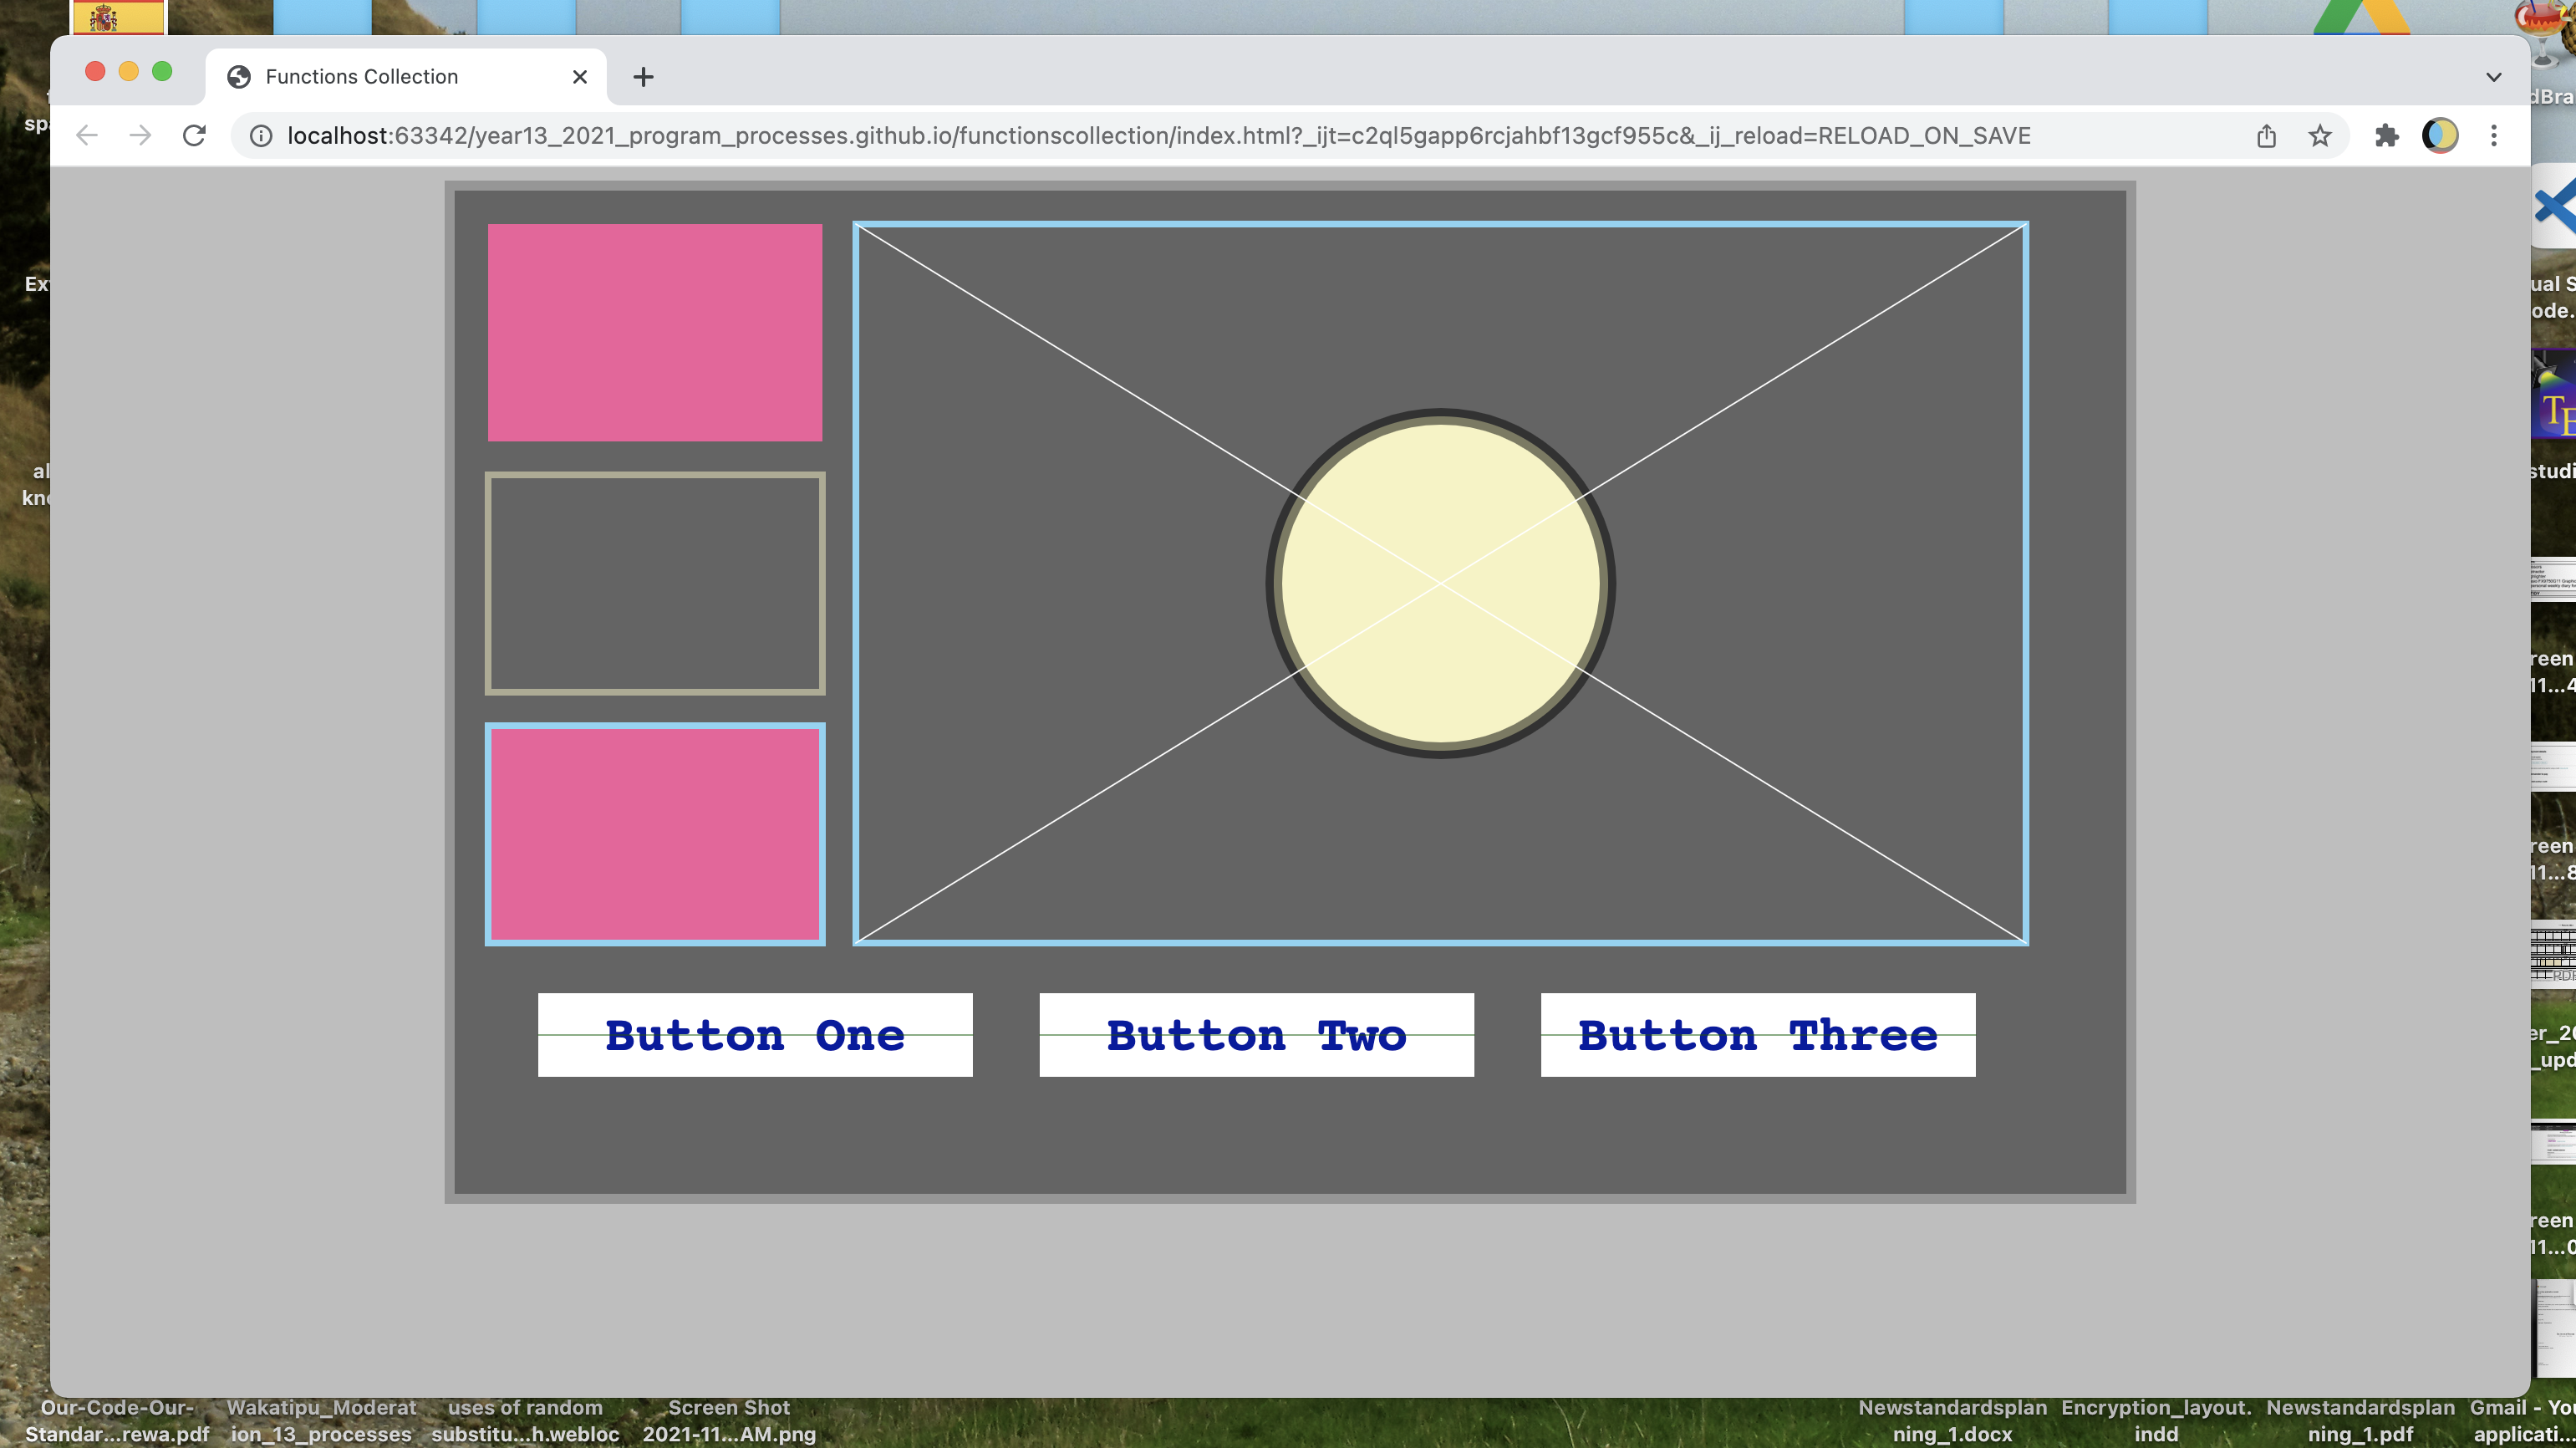
\includegraphics[width=18cm, angle=0, origin=c]{functionscollection/littleinterface.png}
\end{center}
\newpage
\section{Rotations}
\newpage
\section{Objects}
We are intending to introduce animation into our canvas environment.\\
To do so we will need to create objects.\\
At present, it will appear to serve no new purpose, so please be patient. Just about everything we make will be object based from now on.\\
Diagram\\
\lstinputlisting[language=JavaScript, caption=Init file (not shown) ,  linerange={1-4} ]{newobjects/init.js}
\lstinputlisting[language=JavaScript, caption=objectSet file]{newobjects/objectSet.js}
\lstinputlisting[language=HTML, caption=Implementing (using HTML file),  linerange={10-45} ]{newobjects/index.html}
\newpage
\section{Animation Frame}
Set up code
\lstinputlisting[language=JavaScript, caption=init]{animationframe/init.js}
\lstinputlisting[language=JavaScript, caption=objects]{animationframe/objects.js}
\lstinputlisting[language=JavaScript, caption=index ]{animationframe/index_start.html}
\begin{center}
	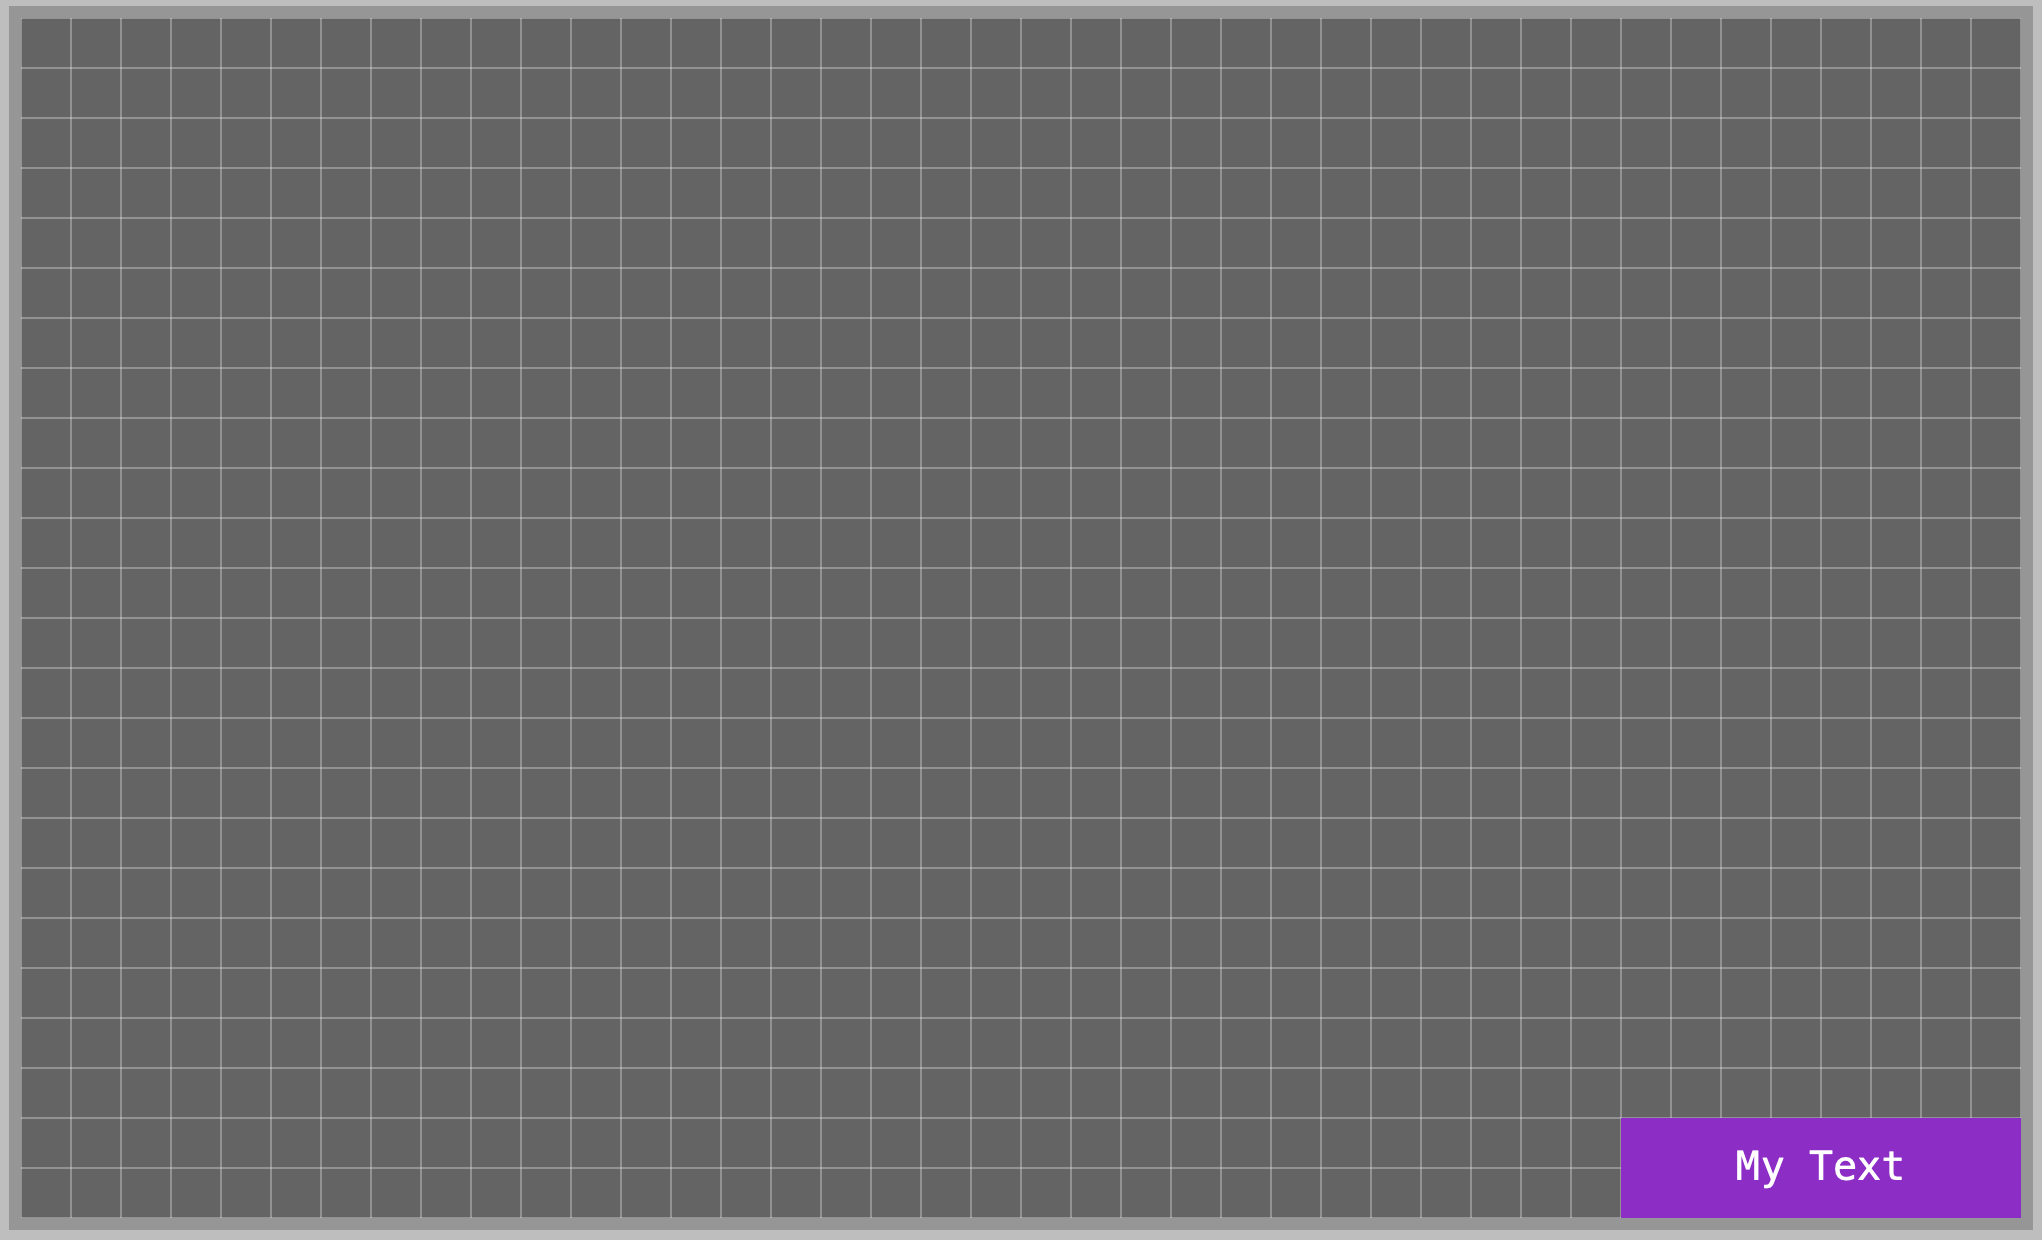
\includegraphics[width=18cm, angle=0, origin=c]{animationframe/start_up.png}
\end{center}
\lstinputlisting[language=JavaScript, caption=index ,   linerange={13-28} ]{animationframe/index.html}
\begin{center}
	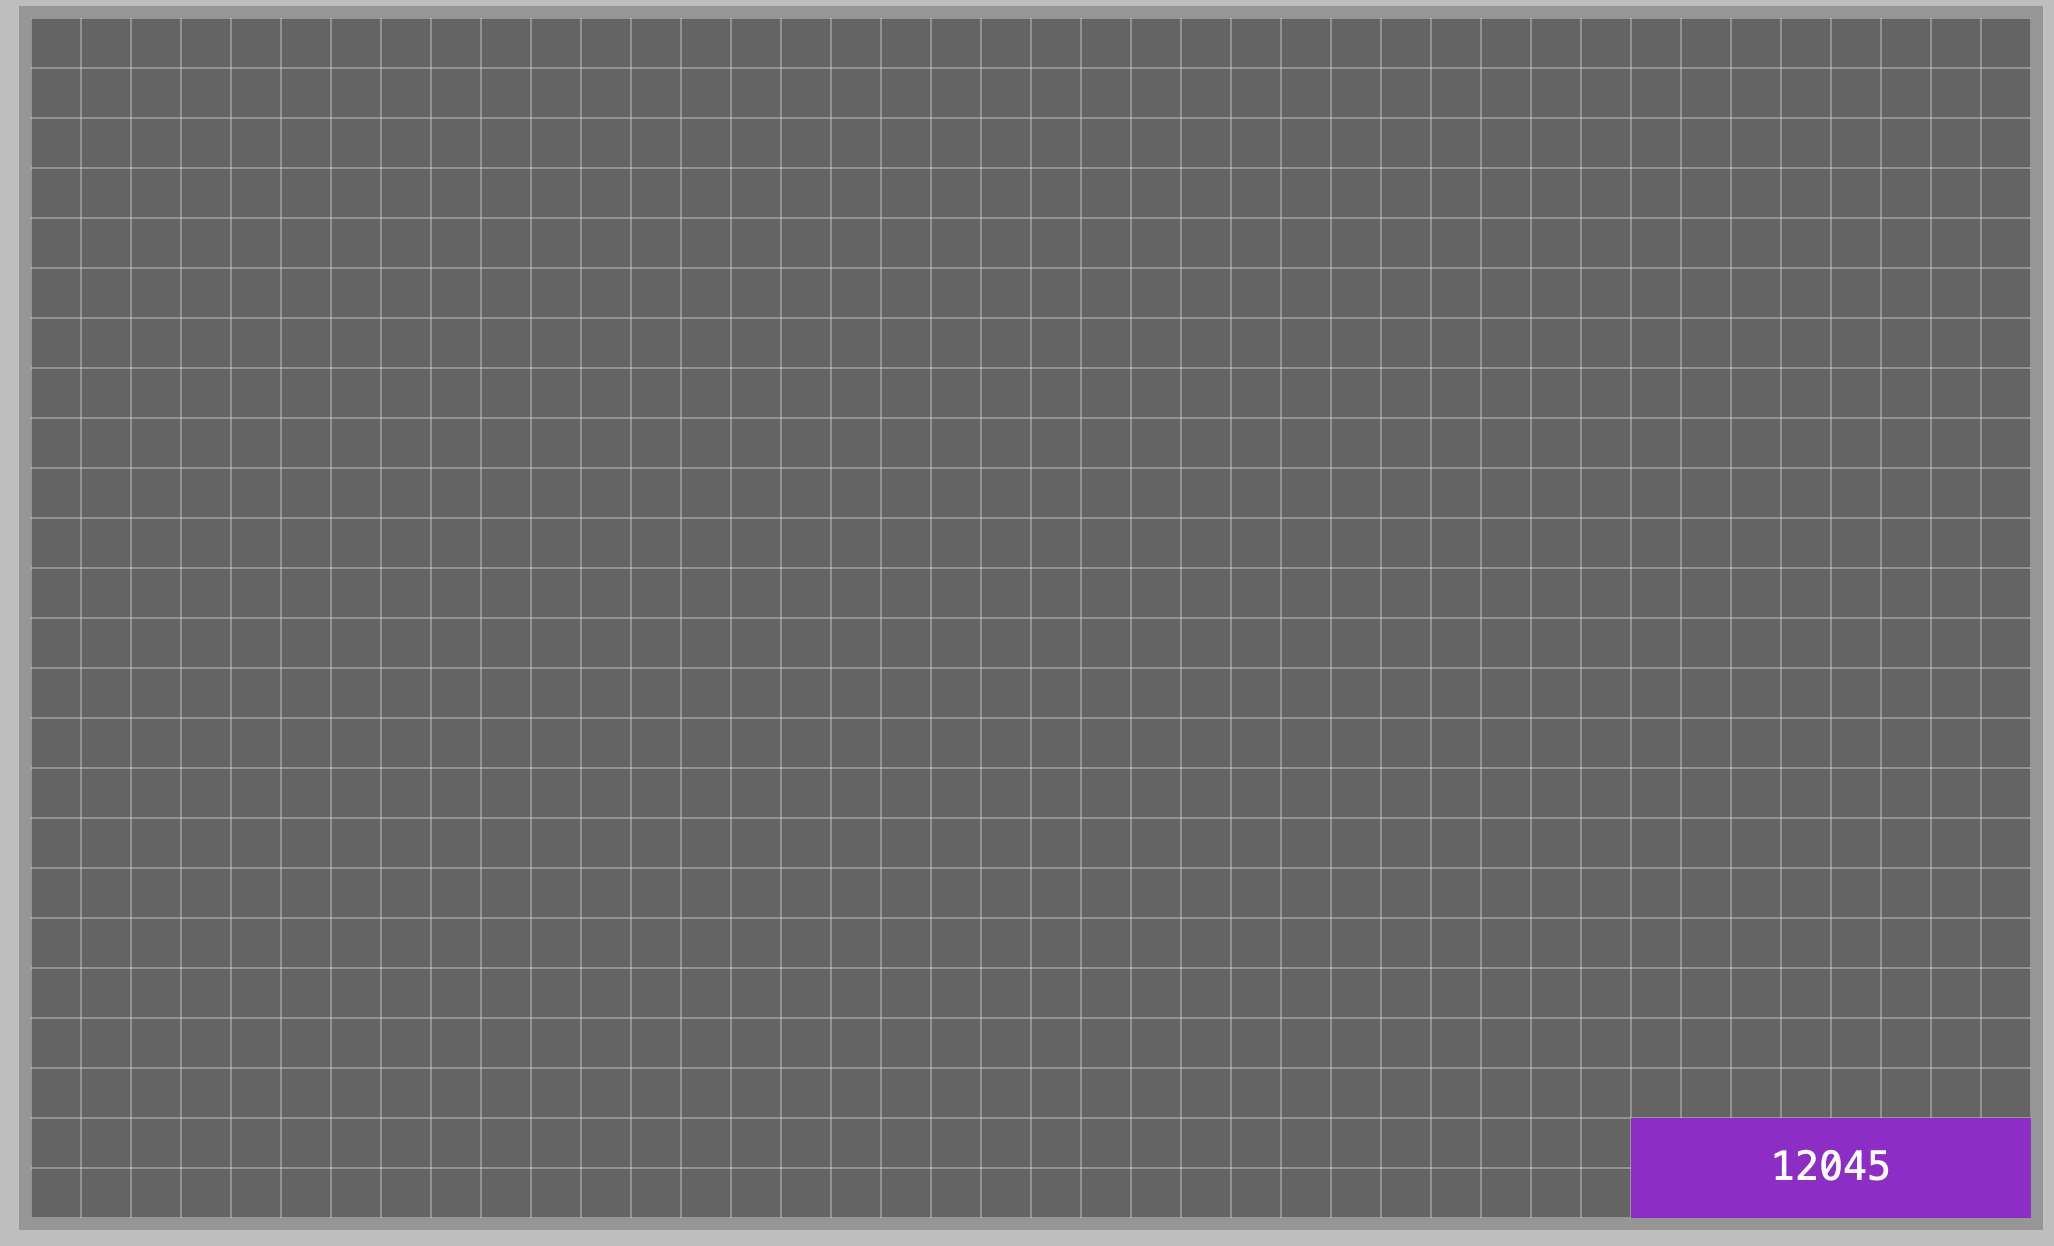
\includegraphics[width=18cm, angle=0, origin=c,]{animationframe/animation_frame_running.png}
\end{center}
\newpage
\section{Animation}
\subsection{Linear Interpolation}
Consider the graph below.\\
The graph runs of a interval of $T$ and moves between a maximum height of $H$ and a minimum of $0$.\\
We could use this to represent a, very simple, motion of a ball going up and down.\\
If we keep repeating the interval, the ball would go up and don indefinitely.\\
The lower case $t$ represents the `time ticks' and is like the $x$ value.\\
The equations for this piecewise graph are given below and you should be able to work these out for yourself.\\

\textbf{The graph has been drawn upside down, so it is like the canvas co-ordinate system}

\begin{center}
\newcommand{\T}{12}
\newcommand{\Hg}{8}
	\begin{tikzpicture}[scale=0.8, yscale = -1]
		\draw[white](0,0) rectangle(10,5);
		\draw[black, thick, ->](0,0)--(\T+1,0)node[right]{$t$};
		\draw[black, thick, ->](0,0)--(0,\Hg+1)node[below]{$y$};;

		\draw[color=blue,very thick,domain=0:\T/2, smooth] plot (\x, { -2*\Hg*(\x)/(\T)  +\Hg});
		\draw[color=blue,very thick,domain=\T/2:\T, smooth] plot (\x, { 2*\Hg*(\x)/(\T)  - \Hg});
	
	
		
		\foreach \y in {0.5,1,...,\Hg}{
				\filldraw[red] (-2,\y) circle[radius=0.1cm];
		}
	%\draw (\T,0) -- (\T,-0.1)node[anchor=north] {\tiny \T};
	\draw (\T,0) -- (\T,-0.1)node[anchor=south] { T};
	\draw (0,\Hg) -- (-0.1,\Hg)node[anchor=east] { H};
	\draw (\T/2,0) -- (\T/2,-0.1)node[anchor=south] {$\frac{T}{2}$};

	\end{tikzpicture}
\end{center}\vspace{0.5cm}
$$\begin{cases}
	\displaystyle y=\frac{-2Ht}{T} + H ~~~,& \displaystyle 0< t \leq \frac{T}{2} \\\\
	\displaystyle y=\frac{2Ht}{T} - H ~~~, &\displaystyle   \frac{T}{2} <x\leq T
\end{cases}
$$\\
We have an animation frame that runs at somewhere between 40 and 60 time ticks per second.\\
So we should be able to implement the functions given about and update the $t$ value, for every tick of the animation frame.
\newpage
Moving Ball Object
\lstinputlisting[language=JavaScript, caption=Moving Ball,   linerange={1-51} ]{animation_frame_interpolation/objects.js}
\begin{center}
	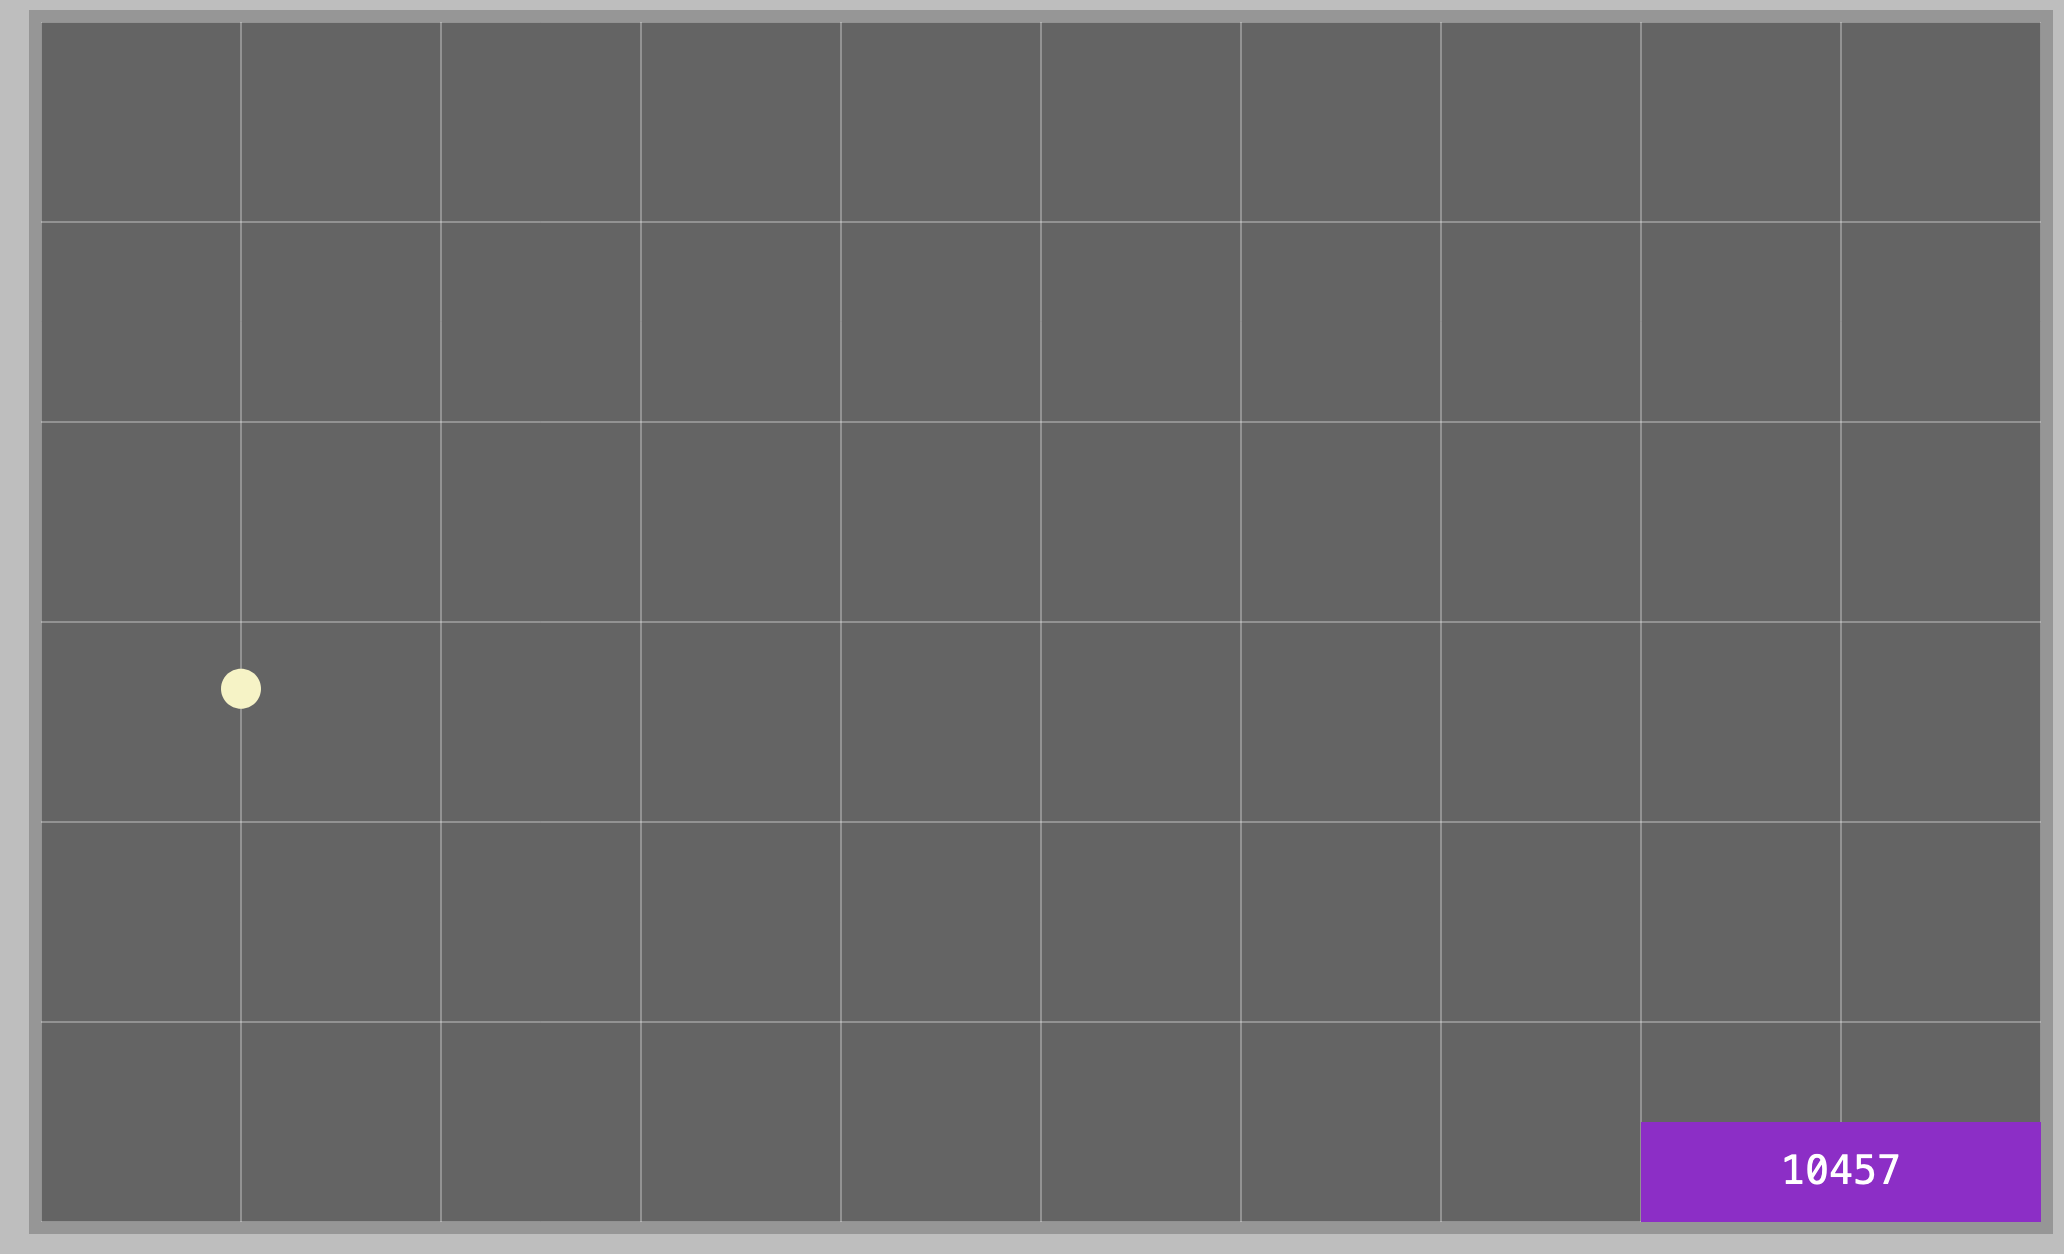
\includegraphics[width=18cm, angle=0, origin=c,]{animation_frame_interpolation/updown.png}
\end{center}
\newpage
We can introduce left right motion.
\lstinputlisting[language=JavaScript, caption=Part of Bothways Moving Ball,   linerange={63-89} ]{animation_frame_interpolation/objects.js}
\begin{center}
	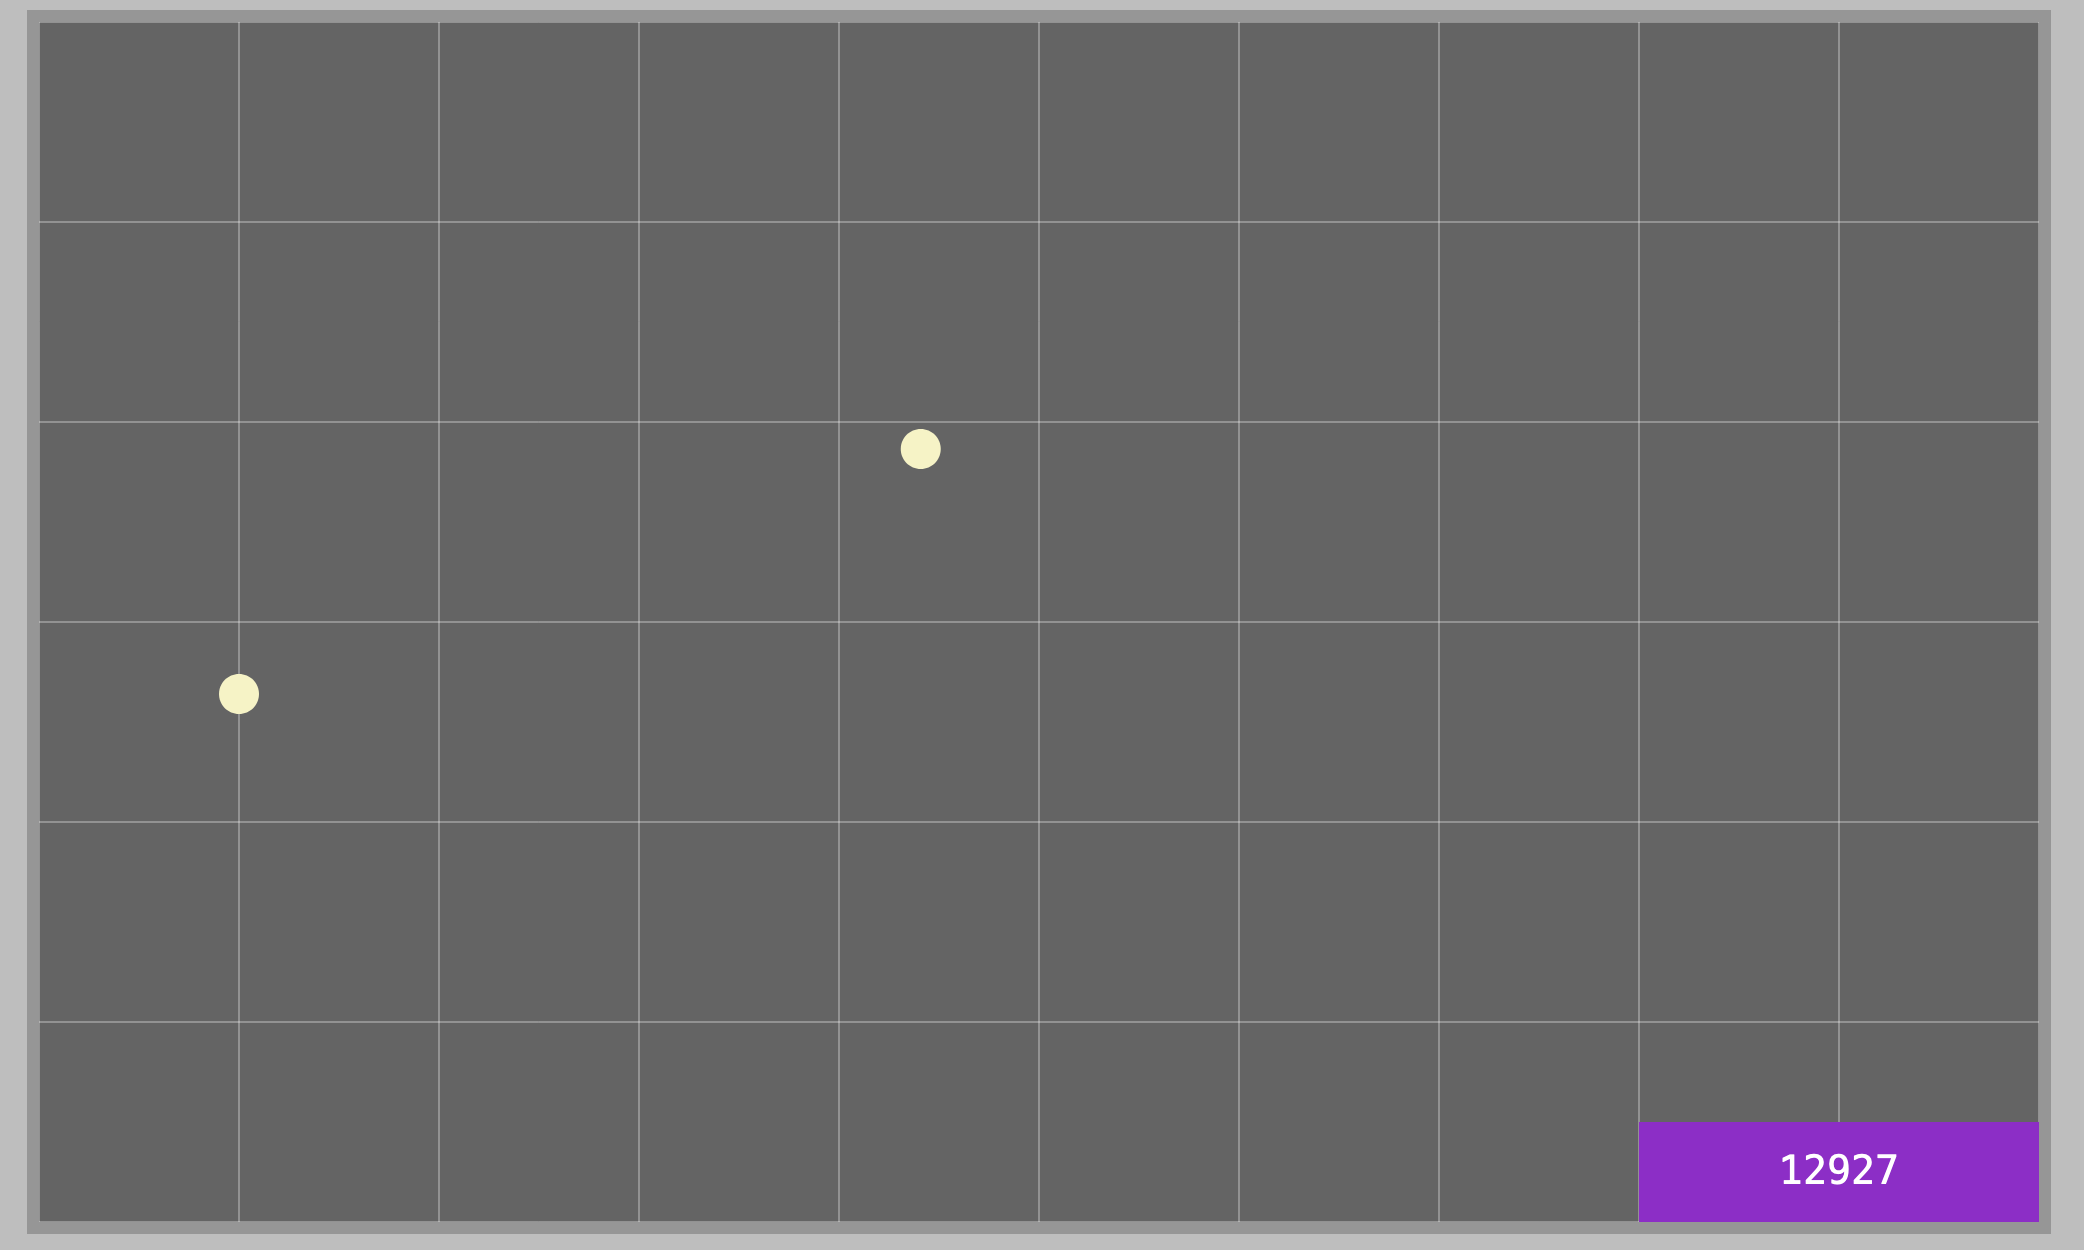
\includegraphics[width=18cm, angle=0, origin=c,]{animation_frame_interpolation/updownlefttright.png}
\end{center}
\newpage
Introduce a whole group (or field) of moving balls.\\
\lstinputlisting[language=JavaScript, caption=Field of moving balls,   linerange={113-166} ]{animation_frame_interpolation/objects.js}
\begin{center}
	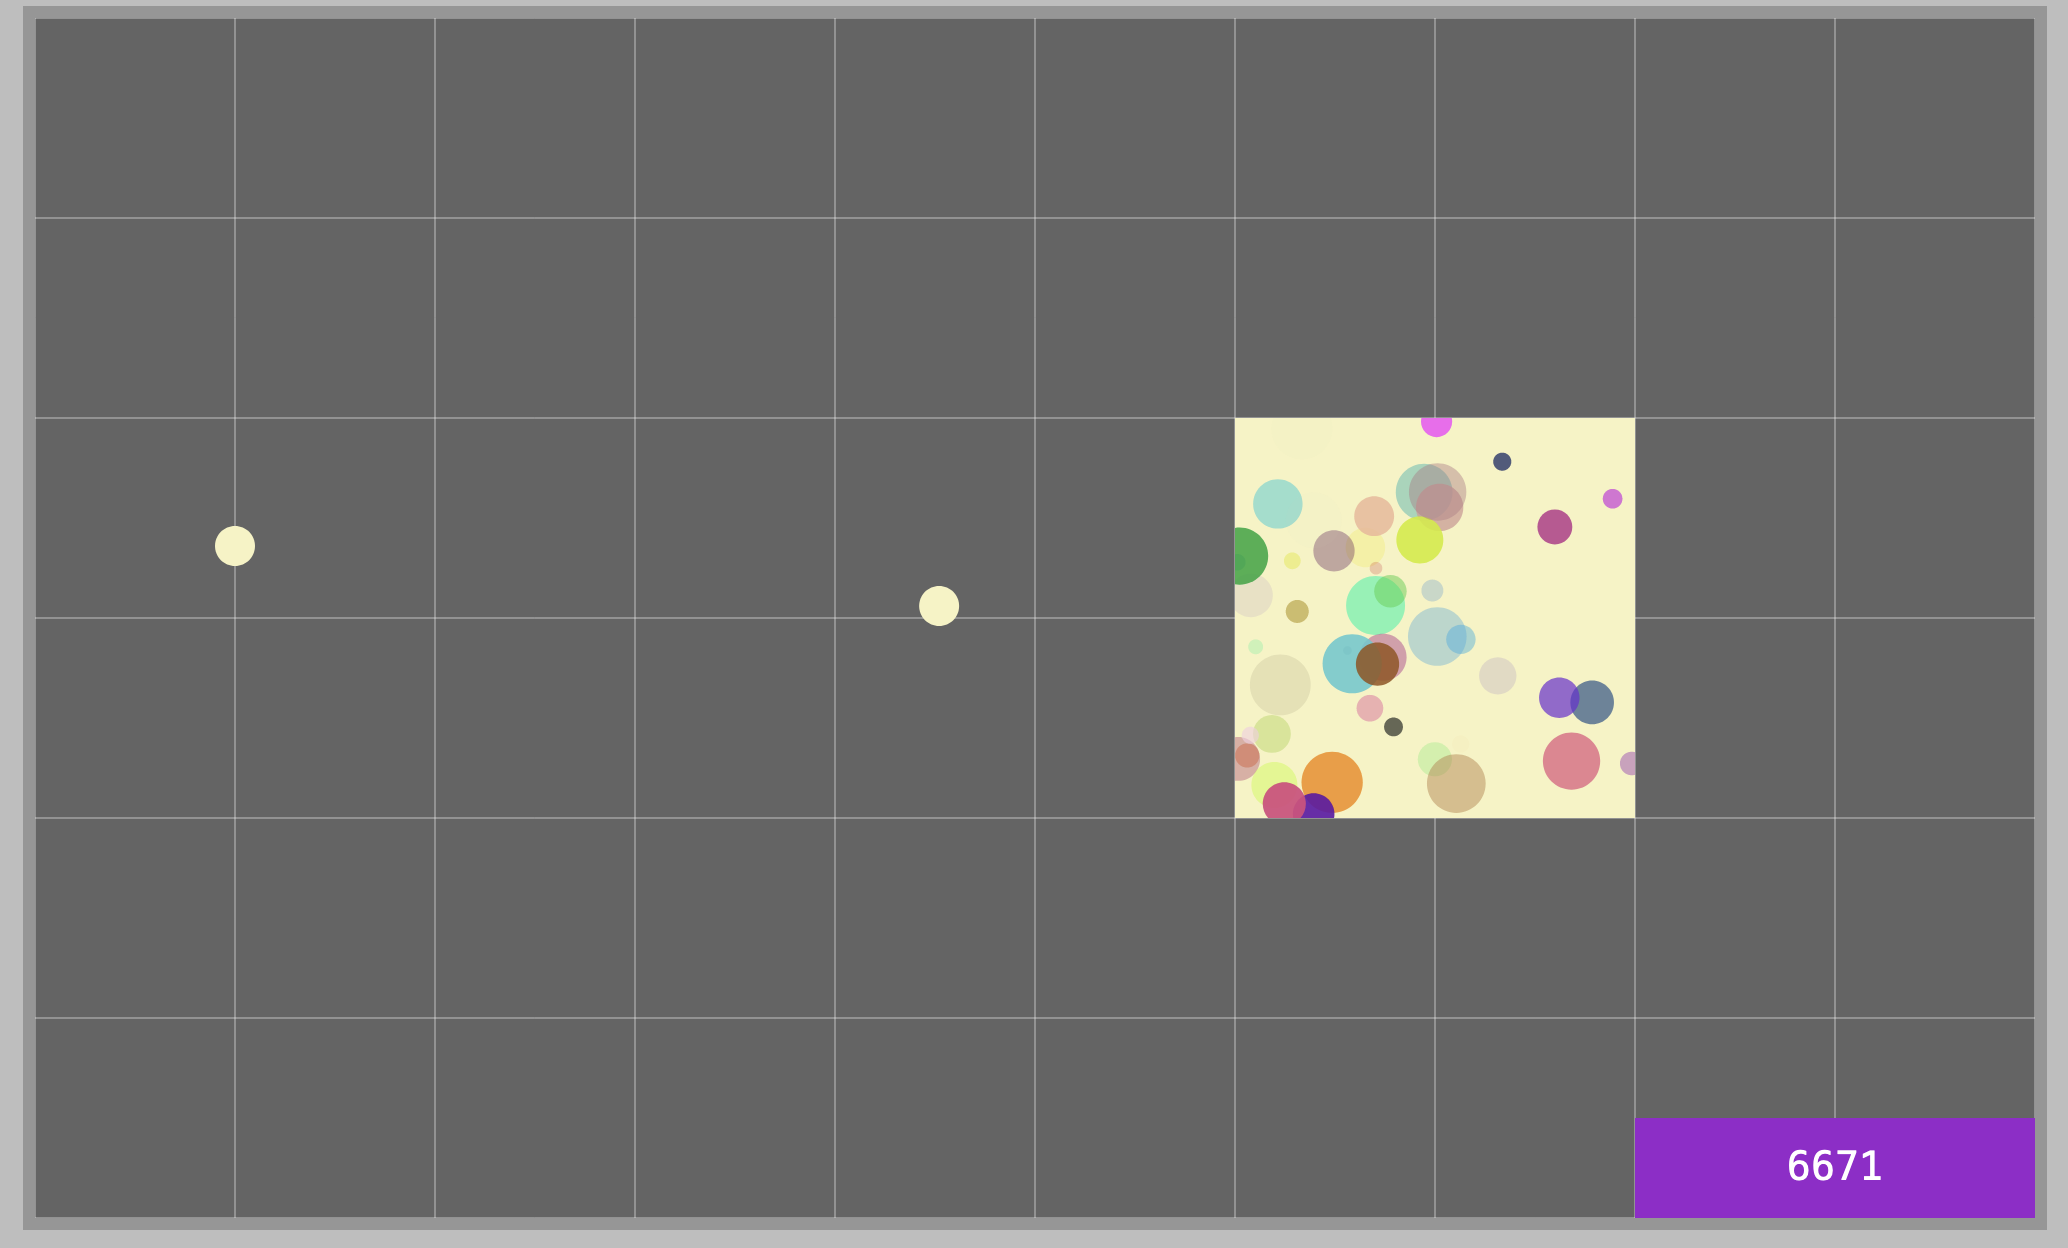
\includegraphics[width=18cm, angle=0, origin=c,]{animation_frame_interpolation/withgroup.png}
\end{center}
\newpage
\subsection{Quadratic Interpolation}
We can follow the same idea using parabolas:
\begin{center}
	\newcommand{\T}{12}
	\newcommand{\Hg}{8}
	\begin{tikzpicture}[scale=0.8, yscale = -1]
		\draw[white](0,0) rectangle(10,5);
		\draw[black, thick, ->](0,0)--(\T+1,0)node[right]{$t$};
		\draw[black, thick, ->](0,0)--(0,\Hg+1)node[below]{$y$};;
		
		\draw[color=blue,very thick,domain=0:\T/2, smooth] plot (\x, { 4*\Hg*(\x)^2 / ( (\T)^2 ) } );
		\draw[color=blue,very thick,domain=\T/2:\T, smooth] plot (\x, { 4*\Hg*(\x - \T)^2 / ( (\T)^2 ) });
		
		
			\newcommand{\Thalf}{6}
		\foreach \y in {0.5,1,...,\Thalf }{
			\filldraw[red] (-2, { 4*\Hg*(\y)^2 / ( (\T)^2 ) } ) circle[radius=0.1cm];
		}
		%\draw (\T,0) -- (\T,-0.1)node[anchor=north] {\tiny \T};
		\draw (\T,0) -- (\T,-0.1)node[anchor=south] { T};
		\draw (0,\Hg) -- (-0.1,\Hg)node[anchor=east] { H};
		\draw (\T/2,0) -- (\T/2,-0.1)node[anchor=south] {$\frac{T}{2}$};
		
	\end{tikzpicture}
\end{center}\vspace{0.5cm}
$$\begin{cases}
	\displaystyle y=\frac{4Ht^2}{T^2} ~~~,& \displaystyle 0< t \leq \frac{T}{2} \\\\
	\displaystyle y=\frac{4H(t-T)^2}{T^2} ~~~, &\displaystyle   \frac{T}{2} <x\leq T
\end{cases}
$$\\
In this case, we would have the up down motion as quadratic, and the the left right as linear.\\\\
Below is the code for a Quadratic Ball Class.\\
Notice how short it is. What's going on here?

\lstinputlisting[language=JavaScript, caption=Quadratic Ball Class,   linerange={187-210} ]{animation_frame_interpolation/objects.js}
\begin{center}
	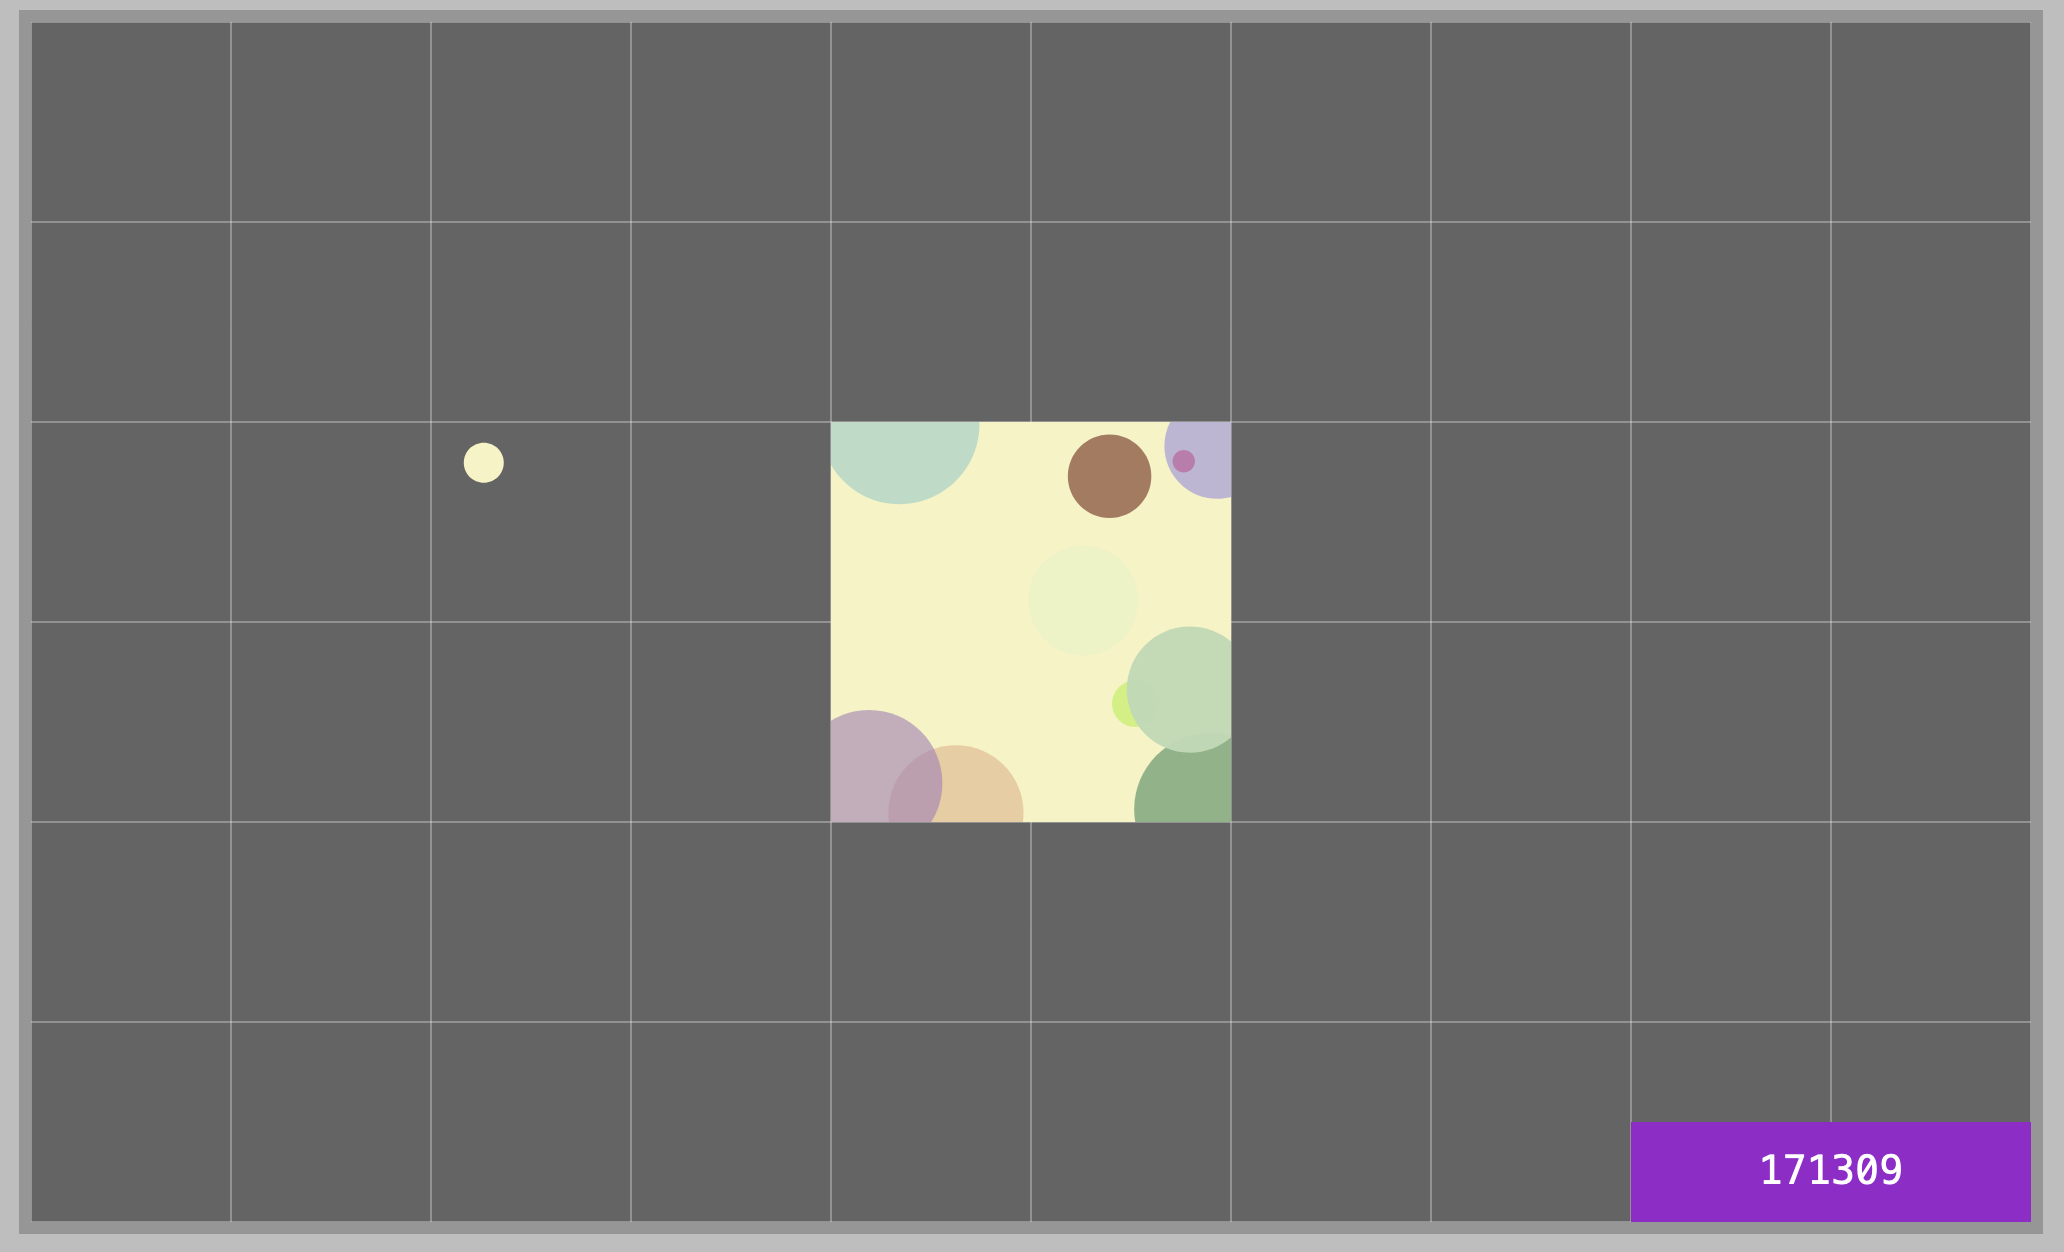
\includegraphics[width=18cm, angle=0, origin=c]{animation_frame_interpolation/quadraticball.png}
\end{center}
A small rewrite has been done on the QuadraticBallGroup Class.\\
This will mean it can be extended in the next section.\\
\lstinputlisting[language=JavaScript, caption=Quadratic Ball Class,   linerange={243-253} ]{animation_frame_interpolation/objects.js}
\newpage
\subsection{Trigonometric  Interpolation}
We can follow the same idea using parabolas:
\begin{center}
	\newcommand{\T}{12}
	\newcommand{\Hg}{8}
	\begin{tikzpicture}[scale=0.8, yscale = -1]
		\draw[white](0,0) rectangle(10,5);
		\draw[black, thick, ->](0,0)--(\T+1,0)node[right]{$t$};
		\draw[black, thick, ->](0,0)--(0,\Hg+1)node[below]{$y$};;
		
		\draw[color=blue,very thick,domain=0:\T, smooth] plot (\x, { (\Hg / 2)*cos( (2*pi / \T )*\x  r ) + \Hg / 2 } );

		
		
		\newcommand{\Thalf}{6}
		\foreach \y in {0, 0.5,1,...,\T}{
			\filldraw[red] (-2, { (\Hg / 2)*cos( (2*pi / \T )*\y  r ) + \Hg / 2 } ) circle[radius=0.1cm];
		}
		%\draw (\T,0) -- (\T,-0.1)node[anchor=north] {\tiny \T};
		\draw (\T,0) -- (\T,-0.1)node[anchor=south] { T};
		\draw (0,\Hg) -- (-0.1,\Hg)node[anchor=east] { H};
		\draw (\T/2,0) -- (\T/2,-0.1)node[anchor=south] {$\frac{T}{2}$};
		
	\end{tikzpicture}
\end{center}\vspace{0.5cm}
$$y = \frac{H}{2}\cos( \frac{2\pi}{T}t) +\frac{H}{2}$$

\vspace{1cm}
Complete code for both the TrigBall class and TrigBallGroup class (both are inheriting from the class referred to in the extension).
\lstinputlisting[language=JavaScript, caption=Quadratic Ball Class,   linerange={277-315} ]{animation_frame_interpolation/objects.js}
\begin{center}
	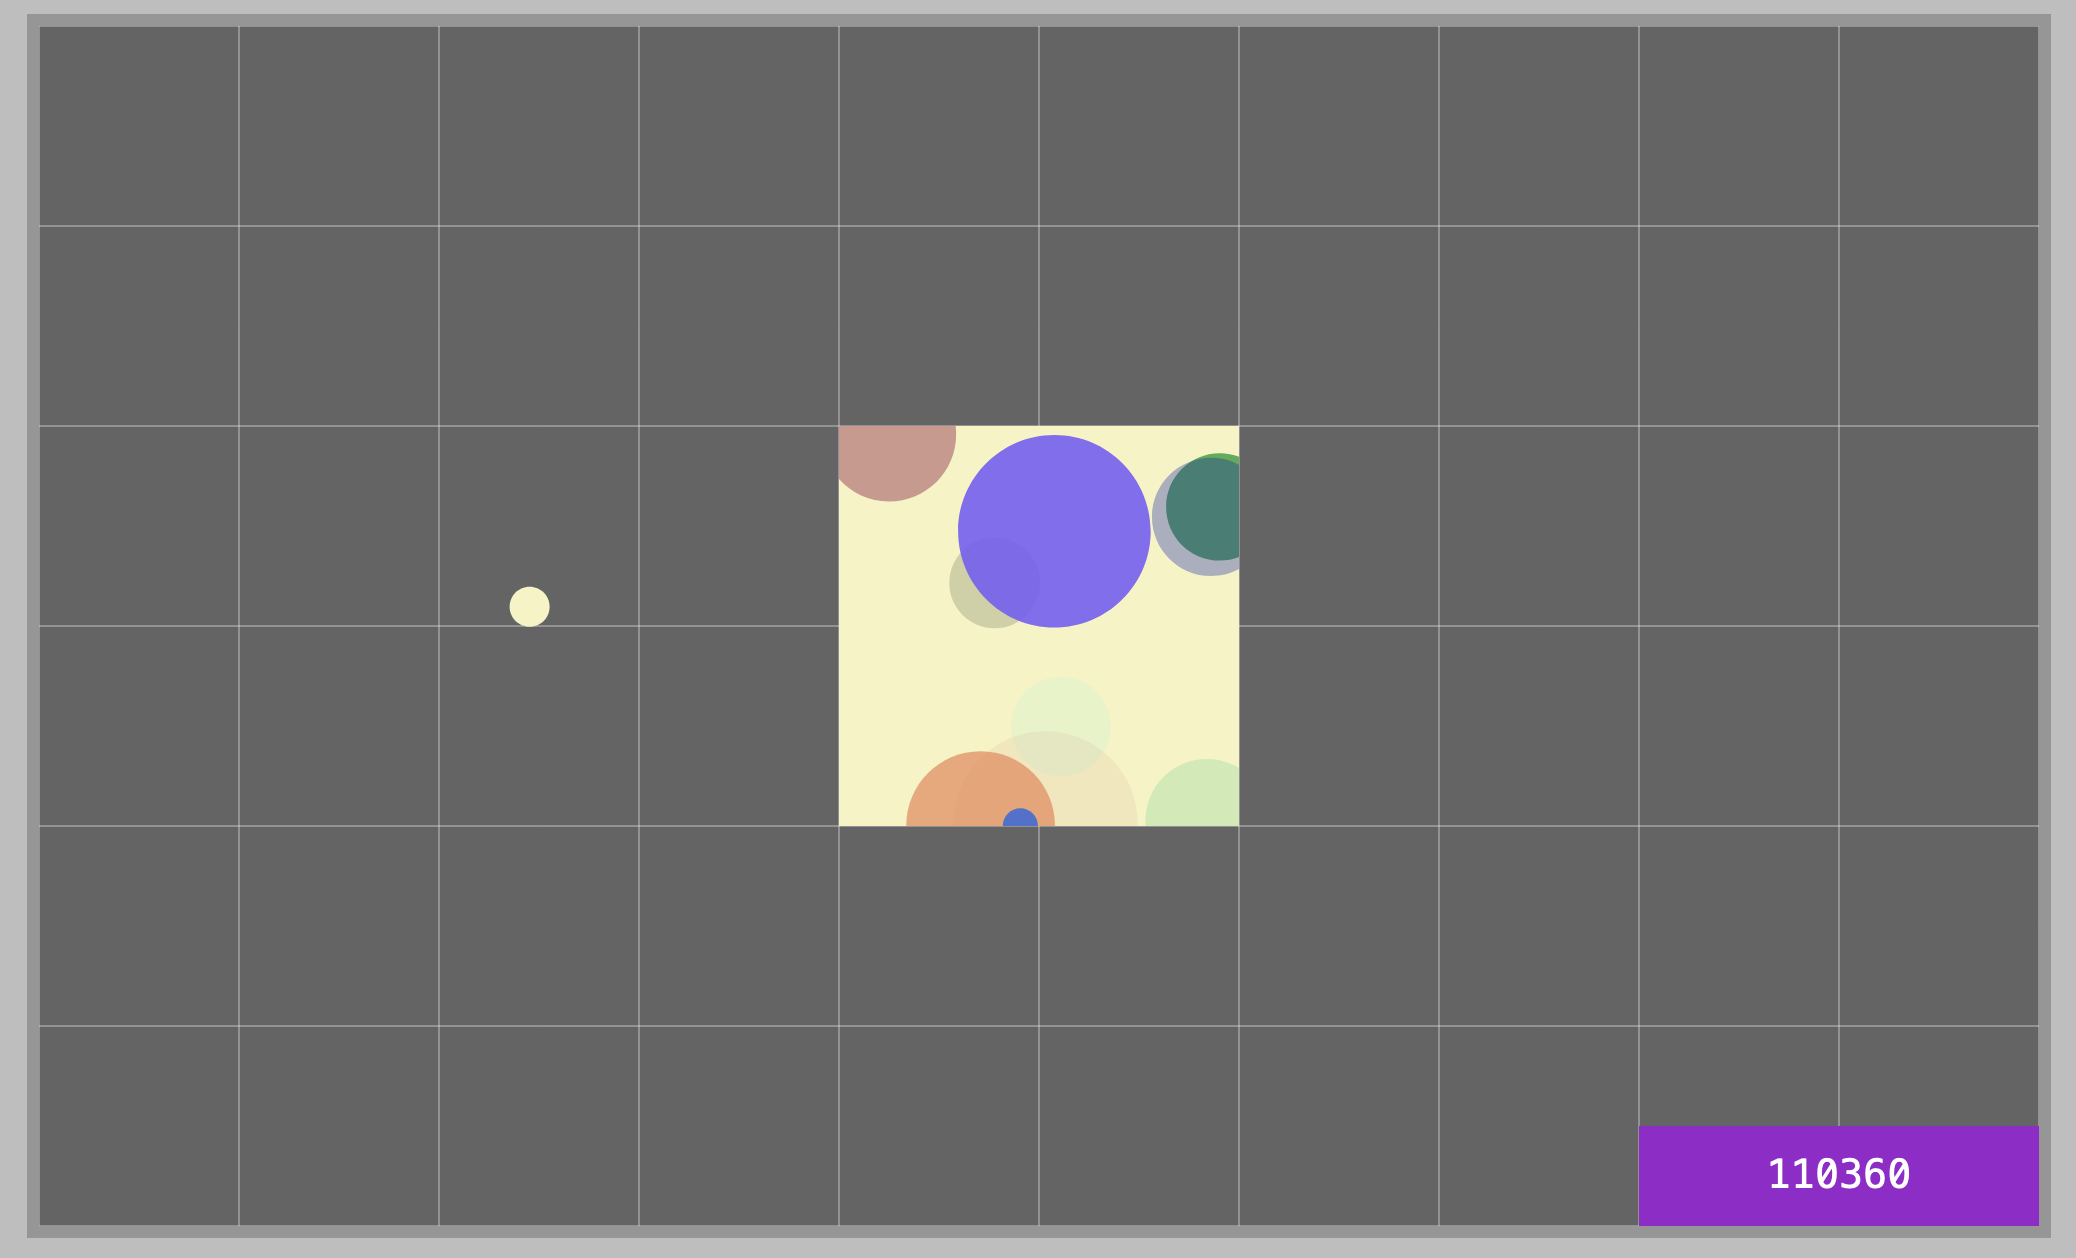
\includegraphics[width=18cm, angle=0, origin=c]{animation_frame_interpolation/trig_balls.png}
\end{center}



\section{Event Handling}
\section{Basic Draggable Point}

\section{Better Draggable Point}



\lstinputlisting[language=JavaScript, caption=Python example ]{slider/point.js}

\section{Buttons}
\end{document}